%% bm.pdf preamble - material merged from previous preamble and current pandoc preamable output
% NOTE: float placement required changes to the source files referenced by bm.tex
% May 28, 2020
%
% Use lualatex to compile - test with MiKTeX 2.9

% uncomment to list all files in log
%\listfiles

\documentclass[12pt]{report}


\usepackage{fontspec}

%\setmainfont[Scale=MatchLowercase]{Lucida Bright}
%\setmonofont{FreeMono}
%\setmonofont{Source Code Pro}
\setmonofont[Scale=MatchLowercase]{Ubuntu Mono}

% short snippets of asian languages
\newfontfamily\myAsian{Noto Serif TC Medium}

\usepackage[headings]{fullpage}

% national use characters 
%\usepackage{inputenc}

% ams mathematical symbols
\usepackage{amsmath,amssymb}

% added to support pandoc highlighting
\usepackage{microtype}

\usepackage{makeidx}

% add index and bibliographies to table of contents
\usepackage[nottoc]{tocbibind}

% postscript courier and times in place of cm fonts
%\usepackage{courier}
%\usepackage{times}

% extended coloring
\usepackage{color}
\usepackage[table,dvipsnames]{xcolor}
\usepackage{colortbl}

% advanced date formating
\usepackage{datetime}

%support pandoc code highlighting
\usepackage{fancyvrb}

% \DefineShortVerb[commandchars=\\\{\}]{\|}
% \DefineVerbatimEnvironment{Highlighting}{Verbatim}{commandchars=\\\{\}}
% % Add ',fontsize=\small' for more characters per line

% tango style colors
% \usepackage{framed}
% \definecolor{shadecolor}{RGB}{255,255,255}
% \newenvironment{Shaded}{\begin{snugshade}}{\end{snugshade}}
% \newcommand{\KeywordTok}[1]{\textcolor[rgb]{0.13,0.29,0.53}{\textbf{{#1}}}}
% \newcommand{\DataTypeTok}[1]{\textcolor[rgb]{0.13,0.29,0.53}{{#1}}}
% \newcommand{\DecValTok}[1]{\textcolor[rgb]{0.00,0.00,0.81}{{#1}}}
% \newcommand{\BaseNTok}[1]{\textcolor[rgb]{0.00,0.00,0.81}{{#1}}}
% \newcommand{\FloatTok}[1]{\textcolor[rgb]{0.00,0.00,0.81}{{#1}}}
% \newcommand{\CharTok}[1]{\textcolor[rgb]{0.31,0.60,0.02}{{#1}}}
% \newcommand{\StringTok}[1]{\textcolor[rgb]{0.31,0.60,0.02}{{#1}}}
% \newcommand{\CommentTok}[1]{\textcolor[rgb]{0.56,0.35,0.01}{\textit{{#1}}}}
% \newcommand{\OtherTok}[1]{\textcolor[rgb]{0.56,0.35,0.01}{{#1}}}
% \newcommand{\AlertTok}[1]{\textcolor[rgb]{0.94,0.16,0.16}{{#1}}}
% \newcommand{\FunctionTok}[1]{\textcolor[rgb]{0.00,0.00,0.00}{{#1}}}
% \newcommand{\RegionMarkerTok}[1]{{#1}}
% \newcommand{\ErrorTok}[1]{\textbf{{#1}}}
% \newcommand{\NormalTok}[1]{{#1}}

% %espresso style colors
% \usepackage{framed}
% \definecolor{shadecolor}{RGB}{42,33,28}
% \newenvironment{Shaded}{\begin{snugshade}}{\end{snugshade}}
% \newcommand{\KeywordTok}[1]{\textcolor[rgb]{0.26,0.66,0.93}{\textbf{{#1}}}}
% \newcommand{\DataTypeTok}[1]{\textcolor[rgb]{0.74,0.68,0.62}{\underline{{#1}}}}
% \newcommand{\DecValTok}[1]{\textcolor[rgb]{0.27,0.67,0.26}{{#1}}}
% \newcommand{\BaseNTok}[1]{\textcolor[rgb]{0.27,0.67,0.26}{{#1}}}
% \newcommand{\FloatTok}[1]{\textcolor[rgb]{0.27,0.67,0.26}{{#1}}}
% \newcommand{\CharTok}[1]{\textcolor[rgb]{0.02,0.61,0.04}{{#1}}}
% \newcommand{\StringTok}[1]{\textcolor[rgb]{0.02,0.61,0.04}{{#1}}}
% \newcommand{\CommentTok}[1]{\textcolor[rgb]{0.00,0.40,1.00}{\textit{{#1}}}}
% \newcommand{\OtherTok}[1]{\textcolor[rgb]{0.74,0.68,0.62}{{#1}}}
% \newcommand{\AlertTok}[1]{\textcolor[rgb]{1.00,1.00,0.00}{{#1}}}
% \newcommand{\FunctionTok}[1]{\textcolor[rgb]{1.00,0.58,0.35}{\textbf{{#1}}}}
% \newcommand{\RegionMarkerTok}[1]{\textcolor[rgb]{0.74,0.68,0.62}{{#1}}}
% \newcommand{\ErrorTok}[1]{\textcolor[rgb]{0.74,0.68,0.62}{\textbf{{#1}}}}
% \newcommand{\NormalTok}[1]{\textcolor[rgb]{0.74,0.68,0.62}{{#1}}}

% %kete style colors
% \newenvironment{Shaded}{}{}
% \newcommand{\KeywordTok}[1]{\textbf{{#1}}}
% \newcommand{\DataTypeTok}[1]{\textcolor[rgb]{0.50,0.00,0.00}{{#1}}}
% \newcommand{\DecValTok}[1]{\textcolor[rgb]{0.00,0.00,1.00}{{#1}}}
% \newcommand{\BaseNTok}[1]{\textcolor[rgb]{0.00,0.00,1.00}{{#1}}}
% \newcommand{\FloatTok}[1]{\textcolor[rgb]{0.50,0.00,0.50}{{#1}}}
% \newcommand{\CharTok}[1]{\textcolor[rgb]{1.00,0.00,1.00}{{#1}}}
% \newcommand{\StringTok}[1]{\textcolor[rgb]{0.87,0.00,0.00}{{#1}}}
% \newcommand{\CommentTok}[1]{\textcolor[rgb]{0.50,0.50,0.50}{\textit{{#1}}}}
% \newcommand{\OtherTok}[1]{{#1}}
% \newcommand{\AlertTok}[1]{\textcolor[rgb]{0.00,1.00,0.00}{\textbf{{#1}}}}
% \newcommand{\FunctionTok}[1]{\textcolor[rgb]{0.00,0.00,0.50}{{#1}}}
% \newcommand{\RegionMarkerTok}[1]{{#1}}
% \newcommand{\ErrorTok}[1]{\textcolor[rgb]{1.00,0.00,0.00}{\textbf{{#1}}}}
% \newcommand{\NormalTok}[1]{{#1}}
% %end pandoc code hacks

% jodliterate colors
\usepackage{color}
\definecolor{shadecolor}{RGB}{248,248,248}
% j control structures 
\definecolor{keywcolor}{rgb}{0.13,0.29,0.53}
% j explicit arguments x y m n u v
\definecolor{datacolor}{rgb}{0.13,0.29,0.53}
% j numbers - all types see j.xml
\definecolor{decvcolor}{rgb}{0.00,0.00,0.81}
\definecolor{basencolor}{rgb}{0.00,0.00,0.81}
\definecolor{floatcolor}{rgb}{0.00,0.00,0.81}
% j local assignments
\definecolor{charcolor}{rgb}{0.31,0.60,0.02}
\definecolor{stringcolor}{rgb}{0.31,0.60,0.02}
\definecolor{commentcolor}{rgb}{0.56,0.35,0.01}
% primitive adverbs and conjunctions
%\definecolor{othercolor}{rgb}{0.56,0.35,0.01}   
\definecolor{othercolor}{RGB}{0,0,255}
% global assignments
\definecolor{alertcolor}{rgb}{0.94,0.16,0.16}
% primitive J verbs and noun names
\definecolor{funccolor}{rgb}{0.00,0.00,0.00}

% custom colors
\definecolor{CodeBackGround}{cmyk}{0.0,0.0,0,0.05}    % light gray
\definecolor{CodeComment}{rgb}{0,0.50,0.00}           % dark green {0,0.45,0.08}
\definecolor{TableStripes}{gray}{0.9}                 % odd/even background in tables

% Colors for the hyperref package
\definecolor{urlcolor}{rgb}{0,.145,.698}
\definecolor{linkcolor}{rgb}{.71,0.21,0.01}
\definecolor{citecolor}{rgb}{.12,.54,.11}

% % Exact colors from NB
\definecolor{incolor}{HTML}{303F9F}
\definecolor{outcolor}{HTML}{D84315}
\definecolor{cellborder}{HTML}{CFCFCF}
\definecolor{cellbackground}{HTML}{F7F7F7}

% % ANSI colors
\definecolor{ansi-black}{HTML}{3E424D}
\definecolor{ansi-black-intense}{HTML}{282C36}
\definecolor{ansi-red}{HTML}{E75C58}
\definecolor{ansi-red-intense}{HTML}{B22B31}
\definecolor{ansi-green}{HTML}{00A250}
\definecolor{ansi-green-intense}{HTML}{007427}
\definecolor{ansi-yellow}{HTML}{DDB62B}
\definecolor{ansi-yellow-intense}{HTML}{B27D12}
\definecolor{ansi-blue}{HTML}{208FFB}
\definecolor{ansi-blue-intense}{HTML}{0065CA}
\definecolor{ansi-magenta}{HTML}{D160C4}
\definecolor{ansi-magenta-intense}{HTML}{A03196}
\definecolor{ansi-cyan}{HTML}{60C6C8}
\definecolor{ansi-cyan-intense}{HTML}{258F8F}
\definecolor{ansi-white}{HTML}{C5C1B4}
\definecolor{ansi-white-intense}{HTML}{A1A6B2}
\definecolor{ansi-default-inverse-fg}{HTML}{FFFFFF}
\definecolor{ansi-default-inverse-bg}{HTML}{000000}
    

% \usepackage{framed}
% \newenvironment{Shaded}{}{}
% \newcommand{\KeywordTok}[1]{\textcolor{keywcolor}{\textbf{{#1}}}}
% \newcommand{\DataTypeTok}[1]{\textcolor{datacolor}{{#1}}}
% %\newcommand{\DecValTok}[1]{\textcolor{decvcolor}{{#1}}}
% \newcommand{\DecValTok}[1]{{#1}} 
% \newcommand{\BaseNTok}[1]{\textcolor{basencolor}{{#1}}}
% \newcommand{\FloatTok}[1]{\textcolor{floatcolor}{{#1}}}
% \newcommand{\CharTok}[1]{\textcolor{charcolor}{\textbf{{#1}}}}
% \newcommand{\StringTok}[1]{\textcolor{stringcolor}{{#1}}}
% \newcommand{\CommentTok}[1]{\textcolor{commentcolor}{\textit{{#1}}}}
% \newcommand{\OtherTok}[1]{\textcolor{othercolor}{{#1}}} 
% \newcommand{\AlertTok}[1]{\textcolor{alertcolor}{\textbf{{#1}}}}
% %\newcommand{\FunctionTok}[1]{\textcolor{funccolor}{{#1}}}
% \newcommand{\FunctionTok}[1]{{#1}}
% \newcommand{\RegionMarkerTok}[1]{{#1}}
% \newcommand{\ErrorTok}[1]{\textbf{{#1}}}
% \newcommand{\NormalTok}[1]{{#1}}

% The default LaTeX title has an obnoxious amount of whitespace. By default,
% titling removes some of it. It also provides customization options.
\usepackage{titling}

% headers and footers
\usepackage{fancyhdr}
%\pagestyle{fancy}
\pagestyle{plain}

\fancyhead{}
\fancyfoot{}

%\fancyhead[LE,RO]{\slshape \rightmark}
%\fancyhead[LO,RE]{\slshape \leftmark}
\fancyfoot[C]{\thepage}
%\headrulewidth 0.4pt
%\footrulewidth 0 pt

%\addtolength{\headheight}{\baselineskip}

%\lfoot{\emph{Analyze the Data not the Drivel}}
%\rfoot{\emph{\today}}

% subfigure handles figures that contain subfigures
%\usepackage{color,graphicx,subfigure,sidecap}
\usepackage{graphicx,sidecap}
\usepackage{subfigure}
\graphicspath{{./inclusions/}}

% floatflt provides for text wrapping around small figures and tables
\usepackage{floatflt}

% tweak caption formats 
\usepackage{caption} 
\usepackage{sidecap}
%\usepackage{subcaption} % not compatible with subfigure

\usepackage{rotating} % flip tables sideways

% complex footnotes
%\usepackage{bigfoot}

% weird logos \XeLaTeX
\usepackage{metalogo}

\newcommand{\HRule}{\rule{\linewidth}{0.5mm}}

\usepackage[breakable]{tcolorbox}

\usepackage{parskip} % Stop auto-indenting (to mimic markdown behaviour)
    
% Basic figure setup, for now with no caption control since it's done
% automatically by Pandoc (which extracts ![](path) syntax from Markdown).
\usepackage{graphicx}

%\DeclareCaptionFormat{nocaption}{}
%\captionsetup{format=nocaption,aboveskip=0pt,belowskip=0pt}

\usepackage[Export]{adjustbox} % Used to constrain images to a maximum size
\adjustboxset{max size={0.9\linewidth}{0.9\paperheight}}
\usepackage{float}

%\floatplacement{figure}{H} % forces figures to be placed at the correct location

\usepackage{xcolor} % Allow colors to be defined
\usepackage{enumerate} % Needed for markdown enumerations to work
\usepackage{geometry} % Used to adjust the document margins

%\usepackage{amsmath} % Equations
%\usepackage{amssymb} % Equations

\usepackage{textcomp} % defines textquotesingle

% Hack from http://tex.stackexchange.com/a/47451/13684:
\AtBeginDocument{%
	\def\PYZsq{\textquotesingle}% Upright quotes in Pygmentized code
}

\usepackage{upquote} % Upright quotes for verbatim code
\usepackage{eurosym} % defines \euro
\usepackage[mathletters]{ucs} % Extended unicode (utf-8) support

%\usepackage{fancyvrb} % verbatim replacement that allows latex

\usepackage{grffile} % extends the file name processing of package graphics 
					 % to support a larger range
					 
\makeatletter % fix for grffile with XeLaTeX
\def\Gread@@xetex#1{%
  \IfFileExists{"\Gin@base".bb}%
  {\Gread@eps{\Gin@base.bb}}%
  {\Gread@@xetex@aux#1}%
}
\makeatother

% The hyperref package gives us a pdf with properly built
% internal navigation ('pdf bookmarks' for the table of contents,
% internal cross-reference links, web links for URLs, etc.)
\usepackage{hyperref}
% The default LaTeX title has an obnoxious amount of whitespace. By default,
% titling removes some of it. It also provides customization options.
\usepackage{titling}
\usepackage{longtable} % longtable support required by pandoc >1.10
\usepackage{booktabs}  % table support for pandoc > 1.12.2
\usepackage[inline]{enumitem} % IRkernel/repr support (it uses the enumerate* environment)
\usepackage[normalem]{ulem} % ulem is needed to support strikethroughs (\sout)
							% normalem makes italics be italics, not underlines
\usepackage{mathrsfs}

% commands and environments needed by pandoc snippets
% extracted from the output of `pandoc -s`
\providecommand{\tightlist}{%
  \setlength{\itemsep}{0pt}\setlength{\parskip}{0pt}}
  
\DefineVerbatimEnvironment{Highlighting}{Verbatim}{commandchars=\\\{\}}
% Add ',fontsize=\small' for more characters per line
\newenvironment{Shaded}{}{}
\newcommand{\KeywordTok}[1]{\textcolor[rgb]{0.00,0.44,0.13}{\textbf{{#1}}}}
\newcommand{\DataTypeTok}[1]{\textcolor[rgb]{0.56,0.13,0.00}{{#1}}}
\newcommand{\DecValTok}[1]{\textcolor[rgb]{0.25,0.63,0.44}{{#1}}}
\newcommand{\BaseNTok}[1]{\textcolor[rgb]{0.25,0.63,0.44}{{#1}}}
\newcommand{\FloatTok}[1]{\textcolor[rgb]{0.25,0.63,0.44}{{#1}}}
\newcommand{\CharTok}[1]{\textcolor[rgb]{0.25,0.44,0.63}{{#1}}}
\newcommand{\StringTok}[1]{\textcolor[rgb]{0.25,0.44,0.63}{{#1}}}
\newcommand{\CommentTok}[1]{\textcolor[rgb]{0.38,0.63,0.69}{\textit{{#1}}}}
\newcommand{\OtherTok}[1]{\textcolor[rgb]{0.00,0.44,0.13}{{#1}}}
\newcommand{\AlertTok}[1]{\textcolor[rgb]{1.00,0.00,0.00}{\textbf{{#1}}}}
\newcommand{\FunctionTok}[1]{\textcolor[rgb]{0.02,0.16,0.49}{{#1}}}
\newcommand{\RegionMarkerTok}[1]{{#1}}
\newcommand{\ErrorTok}[1]{\textcolor[rgb]{1.00,0.00,0.00}{\textbf{{#1}}}}
\newcommand{\NormalTok}[1]{{#1}}

% Additional commands for more recent versions of Pandoc
\newcommand{\ConstantTok}[1]{\textcolor[rgb]{0.53,0.00,0.00}{{#1}}}
\newcommand{\SpecialCharTok}[1]{\textcolor[rgb]{0.25,0.44,0.63}{{#1}}}
\newcommand{\VerbatimStringTok}[1]{\textcolor[rgb]{0.25,0.44,0.63}{{#1}}}
\newcommand{\SpecialStringTok}[1]{\textcolor[rgb]{0.73,0.40,0.53}{{#1}}}
\newcommand{\ImportTok}[1]{{#1}}
\newcommand{\DocumentationTok}[1]{\textcolor[rgb]{0.73,0.13,0.13}{\textit{{#1}}}}
\newcommand{\AnnotationTok}[1]{\textcolor[rgb]{0.38,0.63,0.69}{\textbf{\textit{{#1}}}}}
\newcommand{\CommentVarTok}[1]{\textcolor[rgb]{0.38,0.63,0.69}{\textbf{\textit{{#1}}}}}
\newcommand{\VariableTok}[1]{\textcolor[rgb]{0.10,0.09,0.49}{{#1}}}
\newcommand{\ControlFlowTok}[1]{\textcolor[rgb]{0.00,0.44,0.13}{\textbf{{#1}}}}
\newcommand{\OperatorTok}[1]{\textcolor[rgb]{0.40,0.40,0.40}{{#1}}}
\newcommand{\BuiltInTok}[1]{{#1}}
\newcommand{\ExtensionTok}[1]{{#1}}
\newcommand{\PreprocessorTok}[1]{\textcolor[rgb]{0.74,0.48,0.00}{{#1}}}
\newcommand{\AttributeTok}[1]{\textcolor[rgb]{0.49,0.56,0.16}{{#1}}}
\newcommand{\InformationTok}[1]{\textcolor[rgb]{0.38,0.63,0.69}{\textbf{\textit{{#1}}}}}
\newcommand{\WarningTok}[1]{\textcolor[rgb]{0.38,0.63,0.69}{\textbf{\textit{{#1}}}}}

% Define a nice break command that doesn't care if a line doesn't already exist.
\def\br{\hspace*{\fill} \\* }
% Math Jax compatibility definitions
\def\gt{>}
\def\lt{<}
\let\Oldtex\TeX
\let\Oldlatex\LaTeX
\renewcommand{\TeX}{\textrm{\Oldtex}}
\renewcommand{\LaTeX}{\textrm{\Oldlatex}}
 
% Pygments definitions
\makeatletter
\def\PY@reset{\let\PY@it=\relax \let\PY@bf=\relax%
    \let\PY@ul=\relax \let\PY@tc=\relax%
    \let\PY@bc=\relax \let\PY@ff=\relax}
\def\PY@tok#1{\csname PY@tok@#1\endcsname}
\def\PY@toks#1+{\ifx\relax#1\empty\else%
    \PY@tok{#1}\expandafter\PY@toks\fi}
\def\PY@do#1{\PY@bc{\PY@tc{\PY@ul{%
    \PY@it{\PY@bf{\PY@ff{#1}}}}}}}
\def\PY#1#2{\PY@reset\PY@toks#1+\relax+\PY@do{#2}}

\expandafter\def\csname PY@tok@w\endcsname{\def\PY@tc##1{\textcolor[rgb]{0.73,0.73,0.73}{##1}}}
\expandafter\def\csname PY@tok@c\endcsname{\let\PY@it=\textit\def\PY@tc##1{\textcolor[rgb]{0.25,0.50,0.50}{##1}}}
\expandafter\def\csname PY@tok@cp\endcsname{\def\PY@tc##1{\textcolor[rgb]{0.74,0.48,0.00}{##1}}}
\expandafter\def\csname PY@tok@k\endcsname{\let\PY@bf=\textbf\def\PY@tc##1{\textcolor[rgb]{0.00,0.50,0.00}{##1}}}
\expandafter\def\csname PY@tok@kp\endcsname{\def\PY@tc##1{\textcolor[rgb]{0.00,0.50,0.00}{##1}}}
\expandafter\def\csname PY@tok@kt\endcsname{\def\PY@tc##1{\textcolor[rgb]{0.69,0.00,0.25}{##1}}}
\expandafter\def\csname PY@tok@o\endcsname{\def\PY@tc##1{\textcolor[rgb]{0.40,0.40,0.40}{##1}}}
\expandafter\def\csname PY@tok@ow\endcsname{\let\PY@bf=\textbf\def\PY@tc##1{\textcolor[rgb]{0.67,0.13,1.00}{##1}}}
\expandafter\def\csname PY@tok@nb\endcsname{\def\PY@tc##1{\textcolor[rgb]{0.00,0.50,0.00}{##1}}}
\expandafter\def\csname PY@tok@nf\endcsname{\def\PY@tc##1{\textcolor[rgb]{0.00,0.00,1.00}{##1}}}
\expandafter\def\csname PY@tok@nc\endcsname{\let\PY@bf=\textbf\def\PY@tc##1{\textcolor[rgb]{0.00,0.00,1.00}{##1}}}
\expandafter\def\csname PY@tok@nn\endcsname{\let\PY@bf=\textbf\def\PY@tc##1{\textcolor[rgb]{0.00,0.00,1.00}{##1}}}
\expandafter\def\csname PY@tok@ne\endcsname{\let\PY@bf=\textbf\def\PY@tc##1{\textcolor[rgb]{0.82,0.25,0.23}{##1}}}
\expandafter\def\csname PY@tok@nv\endcsname{\def\PY@tc##1{\textcolor[rgb]{0.10,0.09,0.49}{##1}}}
\expandafter\def\csname PY@tok@no\endcsname{\def\PY@tc##1{\textcolor[rgb]{0.53,0.00,0.00}{##1}}}
\expandafter\def\csname PY@tok@nl\endcsname{\def\PY@tc##1{\textcolor[rgb]{0.63,0.63,0.00}{##1}}}
\expandafter\def\csname PY@tok@ni\endcsname{\let\PY@bf=\textbf\def\PY@tc##1{\textcolor[rgb]{0.60,0.60,0.60}{##1}}}
\expandafter\def\csname PY@tok@na\endcsname{\def\PY@tc##1{\textcolor[rgb]{0.49,0.56,0.16}{##1}}}
\expandafter\def\csname PY@tok@nt\endcsname{\let\PY@bf=\textbf\def\PY@tc##1{\textcolor[rgb]{0.00,0.50,0.00}{##1}}}
\expandafter\def\csname PY@tok@nd\endcsname{\def\PY@tc##1{\textcolor[rgb]{0.67,0.13,1.00}{##1}}}
\expandafter\def\csname PY@tok@s\endcsname{\def\PY@tc##1{\textcolor[rgb]{0.73,0.13,0.13}{##1}}}
\expandafter\def\csname PY@tok@sd\endcsname{\let\PY@it=\textit\def\PY@tc##1{\textcolor[rgb]{0.73,0.13,0.13}{##1}}}
\expandafter\def\csname PY@tok@si\endcsname{\let\PY@bf=\textbf\def\PY@tc##1{\textcolor[rgb]{0.73,0.40,0.53}{##1}}}
\expandafter\def\csname PY@tok@se\endcsname{\let\PY@bf=\textbf\def\PY@tc##1{\textcolor[rgb]{0.73,0.40,0.13}{##1}}}
\expandafter\def\csname PY@tok@sr\endcsname{\def\PY@tc##1{\textcolor[rgb]{0.73,0.40,0.53}{##1}}}
\expandafter\def\csname PY@tok@ss\endcsname{\def\PY@tc##1{\textcolor[rgb]{0.10,0.09,0.49}{##1}}}
\expandafter\def\csname PY@tok@sx\endcsname{\def\PY@tc##1{\textcolor[rgb]{0.00,0.50,0.00}{##1}}}
\expandafter\def\csname PY@tok@m\endcsname{\def\PY@tc##1{\textcolor[rgb]{0.40,0.40,0.40}{##1}}}
\expandafter\def\csname PY@tok@gh\endcsname{\let\PY@bf=\textbf\def\PY@tc##1{\textcolor[rgb]{0.00,0.00,0.50}{##1}}}
\expandafter\def\csname PY@tok@gu\endcsname{\let\PY@bf=\textbf\def\PY@tc##1{\textcolor[rgb]{0.50,0.00,0.50}{##1}}}
\expandafter\def\csname PY@tok@gd\endcsname{\def\PY@tc##1{\textcolor[rgb]{0.63,0.00,0.00}{##1}}}
\expandafter\def\csname PY@tok@gi\endcsname{\def\PY@tc##1{\textcolor[rgb]{0.00,0.63,0.00}{##1}}}
\expandafter\def\csname PY@tok@gr\endcsname{\def\PY@tc##1{\textcolor[rgb]{1.00,0.00,0.00}{##1}}}
\expandafter\def\csname PY@tok@ge\endcsname{\let\PY@it=\textit}
\expandafter\def\csname PY@tok@gs\endcsname{\let\PY@bf=\textbf}
\expandafter\def\csname PY@tok@gp\endcsname{\let\PY@bf=\textbf\def\PY@tc##1{\textcolor[rgb]{0.00,0.00,0.50}{##1}}}
\expandafter\def\csname PY@tok@go\endcsname{\def\PY@tc##1{\textcolor[rgb]{0.53,0.53,0.53}{##1}}}
\expandafter\def\csname PY@tok@gt\endcsname{\def\PY@tc##1{\textcolor[rgb]{0.00,0.27,0.87}{##1}}}
\expandafter\def\csname PY@tok@err\endcsname{\def\PY@bc##1{\setlength{\fboxsep}{0pt}\fcolorbox[rgb]{1.00,0.00,0.00}{1,1,1}{\strut ##1}}}
\expandafter\def\csname PY@tok@kc\endcsname{\let\PY@bf=\textbf\def\PY@tc##1{\textcolor[rgb]{0.00,0.50,0.00}{##1}}}
\expandafter\def\csname PY@tok@kd\endcsname{\let\PY@bf=\textbf\def\PY@tc##1{\textcolor[rgb]{0.00,0.50,0.00}{##1}}}
\expandafter\def\csname PY@tok@kn\endcsname{\let\PY@bf=\textbf\def\PY@tc##1{\textcolor[rgb]{0.00,0.50,0.00}{##1}}}
\expandafter\def\csname PY@tok@kr\endcsname{\let\PY@bf=\textbf\def\PY@tc##1{\textcolor[rgb]{0.00,0.50,0.00}{##1}}}
\expandafter\def\csname PY@tok@bp\endcsname{\def\PY@tc##1{\textcolor[rgb]{0.00,0.50,0.00}{##1}}}
\expandafter\def\csname PY@tok@fm\endcsname{\def\PY@tc##1{\textcolor[rgb]{0.00,0.00,1.00}{##1}}}
\expandafter\def\csname PY@tok@vc\endcsname{\def\PY@tc##1{\textcolor[rgb]{0.10,0.09,0.49}{##1}}}
\expandafter\def\csname PY@tok@vg\endcsname{\def\PY@tc##1{\textcolor[rgb]{0.10,0.09,0.49}{##1}}}
\expandafter\def\csname PY@tok@vi\endcsname{\def\PY@tc##1{\textcolor[rgb]{0.10,0.09,0.49}{##1}}}
\expandafter\def\csname PY@tok@vm\endcsname{\def\PY@tc##1{\textcolor[rgb]{0.10,0.09,0.49}{##1}}}
\expandafter\def\csname PY@tok@sa\endcsname{\def\PY@tc##1{\textcolor[rgb]{0.73,0.13,0.13}{##1}}}
\expandafter\def\csname PY@tok@sb\endcsname{\def\PY@tc##1{\textcolor[rgb]{0.73,0.13,0.13}{##1}}}
\expandafter\def\csname PY@tok@sc\endcsname{\def\PY@tc##1{\textcolor[rgb]{0.73,0.13,0.13}{##1}}}
\expandafter\def\csname PY@tok@dl\endcsname{\def\PY@tc##1{\textcolor[rgb]{0.73,0.13,0.13}{##1}}}
\expandafter\def\csname PY@tok@s2\endcsname{\def\PY@tc##1{\textcolor[rgb]{0.73,0.13,0.13}{##1}}}
\expandafter\def\csname PY@tok@sh\endcsname{\def\PY@tc##1{\textcolor[rgb]{0.73,0.13,0.13}{##1}}}
\expandafter\def\csname PY@tok@s1\endcsname{\def\PY@tc##1{\textcolor[rgb]{0.73,0.13,0.13}{##1}}}
\expandafter\def\csname PY@tok@mb\endcsname{\def\PY@tc##1{\textcolor[rgb]{0.40,0.40,0.40}{##1}}}
\expandafter\def\csname PY@tok@mf\endcsname{\def\PY@tc##1{\textcolor[rgb]{0.40,0.40,0.40}{##1}}}
\expandafter\def\csname PY@tok@mh\endcsname{\def\PY@tc##1{\textcolor[rgb]{0.40,0.40,0.40}{##1}}}
\expandafter\def\csname PY@tok@mi\endcsname{\def\PY@tc##1{\textcolor[rgb]{0.40,0.40,0.40}{##1}}}
\expandafter\def\csname PY@tok@il\endcsname{\def\PY@tc##1{\textcolor[rgb]{0.40,0.40,0.40}{##1}}}
\expandafter\def\csname PY@tok@mo\endcsname{\def\PY@tc##1{\textcolor[rgb]{0.40,0.40,0.40}{##1}}}
\expandafter\def\csname PY@tok@ch\endcsname{\let\PY@it=\textit\def\PY@tc##1{\textcolor[rgb]{0.25,0.50,0.50}{##1}}}
\expandafter\def\csname PY@tok@cm\endcsname{\let\PY@it=\textit\def\PY@tc##1{\textcolor[rgb]{0.25,0.50,0.50}{##1}}}
\expandafter\def\csname PY@tok@cpf\endcsname{\let\PY@it=\textit\def\PY@tc##1{\textcolor[rgb]{0.25,0.50,0.50}{##1}}}
\expandafter\def\csname PY@tok@c1\endcsname{\let\PY@it=\textit\def\PY@tc##1{\textcolor[rgb]{0.25,0.50,0.50}{##1}}}
\expandafter\def\csname PY@tok@cs\endcsname{\let\PY@it=\textit\def\PY@tc##1{\textcolor[rgb]{0.25,0.50,0.50}{##1}}}

\def\PYZbs{\char`\\}
\def\PYZus{\char`\_}
\def\PYZob{\char`\{}
\def\PYZcb{\char`\}}
\def\PYZca{\char`\^}
\def\PYZam{\char`\&}
\def\PYZlt{\char`\<}
\def\PYZgt{\char`\>}
\def\PYZsh{\char`\#}
\def\PYZpc{\char`\%}
\def\PYZdl{\char`\$}
\def\PYZhy{\char`\-}
\def\PYZsq{\char`\'}
\def\PYZdq{\char`\"}
\def\PYZti{\char`\~}
% for compatibility with earlier versions
\def\PYZat{@}
\def\PYZlb{[}
\def\PYZrb{]}
\makeatother

% For linebreaks inside Verbatim environment from package fancyvrb. 
\makeatletter
	\newbox\Wrappedcontinuationbox 
	\newbox\Wrappedvisiblespacebox 
	\newcommand*\Wrappedvisiblespace {\textcolor{red}{\textvisiblespace}} 
	\newcommand*\Wrappedcontinuationsymbol {\textcolor{red}{\llap{\tiny$\m@th\hookrightarrow$}}} 
	\newcommand*\Wrappedcontinuationindent {3ex } 
	\newcommand*\Wrappedafterbreak {\kern\Wrappedcontinuationindent\copy\Wrappedcontinuationbox} 
	% Take advantage of the already applied Pygments mark-up to insert 
	% potential linebreaks for TeX processing. 
	%        {, <, #, %, $, ' and ": go to next line. 
	%        _, }, ^, &, >, - and ~: stay at end of broken line. 
	% Use of \textquotesingle for straight quote. 
	\newcommand*\Wrappedbreaksatspecials {% 
		\def\PYGZus{\discretionary{\char`\_}{\Wrappedafterbreak}{\char`\_}}% 
		\def\PYGZob{\discretionary{}{\Wrappedafterbreak\char`\{}{\char`\{}}% 
		\def\PYGZcb{\discretionary{\char`\}}{\Wrappedafterbreak}{\char`\}}}% 
		\def\PYGZca{\discretionary{\char`\^}{\Wrappedafterbreak}{\char`\^}}% 
		\def\PYGZam{\discretionary{\char`\&}{\Wrappedafterbreak}{\char`\&}}% 
		\def\PYGZlt{\discretionary{}{\Wrappedafterbreak\char`\<}{\char`\<}}% 
		\def\PYGZgt{\discretionary{\char`\>}{\Wrappedafterbreak}{\char`\>}}% 
		\def\PYGZsh{\discretionary{}{\Wrappedafterbreak\char`\#}{\char`\#}}% 
		\def\PYGZpc{\discretionary{}{\Wrappedafterbreak\char`\%}{\char`\%}}% 
		\def\PYGZdl{\discretionary{}{\Wrappedafterbreak\char`\$}{\char`\$}}% 
		\def\PYGZhy{\discretionary{\char`\-}{\Wrappedafterbreak}{\char`\-}}% 
		\def\PYGZsq{\discretionary{}{\Wrappedafterbreak\textquotesingle}{\textquotesingle}}% 
		\def\PYGZdq{\discretionary{}{\Wrappedafterbreak\char`\"}{\char`\"}}% 
		\def\PYGZti{\discretionary{\char`\~}{\Wrappedafterbreak}{\char`\~}}% 
	} 
	% Some characters . , ; ? ! / are not pygmentized. 
	% This macro makes them "active" and they will insert potential linebreaks 
	\newcommand*\Wrappedbreaksatpunct {% 
		\lccode`\~`\.\lowercase{\def~}{\discretionary{\hbox{\char`\.}}{\Wrappedafterbreak}{\hbox{\char`\.}}}% 
		\lccode`\~`\,\lowercase{\def~}{\discretionary{\hbox{\char`\,}}{\Wrappedafterbreak}{\hbox{\char`\,}}}% 
		\lccode`\~`\;\lowercase{\def~}{\discretionary{\hbox{\char`\;}}{\Wrappedafterbreak}{\hbox{\char`\;}}}% 
		\lccode`\~`\:\lowercase{\def~}{\discretionary{\hbox{\char`\:}}{\Wrappedafterbreak}{\hbox{\char`\:}}}% 
		\lccode`\~`\?\lowercase{\def~}{\discretionary{\hbox{\char`\?}}{\Wrappedafterbreak}{\hbox{\char`\?}}}% 
		\lccode`\~`\!\lowercase{\def~}{\discretionary{\hbox{\char`\!}}{\Wrappedafterbreak}{\hbox{\char`\!}}}% 
		\lccode`\~`\/\lowercase{\def~}{\discretionary{\hbox{\char`\/}}{\Wrappedafterbreak}{\hbox{\char`\/}}}% 
		\catcode`\.\active
		\catcode`\,\active 
		\catcode`\;\active
		\catcode`\:\active
		\catcode`\?\active
		\catcode`\!\active
		\catcode`\/\active 
		\lccode`\~`\~ 	
	}
\makeatother

\let\OriginalVerbatim=\Verbatim
\makeatletter
\renewcommand{\Verbatim}[1][1]{%
	%\parskip\z@skip
	\sbox\Wrappedcontinuationbox {\Wrappedcontinuationsymbol}%
	\sbox\Wrappedvisiblespacebox {\FV@SetupFont\Wrappedvisiblespace}%
	\def\FancyVerbFormatLine ##1{\hsize\linewidth
		\vtop{\raggedright\hyphenpenalty\z@\exhyphenpenalty\z@
			\doublehyphendemerits\z@\finalhyphendemerits\z@
			\strut ##1\strut}%
	}%
	% If the linebreak is at a space, the latter will be displayed as visible
	% space at end of first line, and a continuation symbol starts next line.
	% Stretch/shrink are however usually zero for typewriter font.
	\def\FV@Space {%
		\nobreak\hskip\z@ plus\fontdimen3\font minus\fontdimen4\font
		\discretionary{\copy\Wrappedvisiblespacebox}{\Wrappedafterbreak}
		{\kern\fontdimen2\font}%
	}%
	
	% Allow breaks at special characters using \PYG... macros.
	\Wrappedbreaksatspecials
	% Breaks at punctuation characters . , ; ? ! and / need catcode=\active 	
	\OriginalVerbatim[#1,codes*=\Wrappedbreaksatpunct]%
}
\makeatother


% prompt
\makeatletter
\newcommand{\boxspacing}{\kern\kvtcb@left@rule\kern\kvtcb@boxsep}
\makeatother
\newcommand{\prompt}[4]{
	\ttfamily\llap{{\color{#2}[#3]:\hspace{3pt}#4}}\vspace{-\baselineskip}
}
    

% Prevent overflowing lines due to hard-to-break entities
\sloppy 

% Setup hyperref package
\hypersetup{
  breaklinks=true,  % so long urls are correctly broken across lines
  colorlinks=true,
  urlcolor=urlcolor,
  linkcolor=linkcolor,
  citecolor=citecolor,
  pdfauthor={John D. Baker},
  pdftitle={Analyze the Data not the Drivel},
  pdfsubject={Blog},
  pdfcreator={MikTeX+LaTeXe},
  pdfkeywords={blog,wordpress},
  }
  
% Slightly bigger margins than the latex defaults
% \geometry{verbose,tmargin=1in,bmargin=1in,lmargin=1in,rmargin=1in}  

%\usepackage{wrapfig}

% source code listings
\usepackage{listings}

\lstdefinelanguage{bat}
{morekeywords={echo,title,pushd,popd,setlocal,endlocal,off,if,not,exist,set,goto,pause},
sensitive=True,
morecomment=[l]{rem}
}

\lstdefinelanguage{jdoc}
{
morekeywords={},
otherkeywords={assert.,break.,continue.,for.,do.,if.,else.,elseif.,return.,select.,end.
,while.,whilst.,throw.,catch.,catchd.,catcht.,try.,case.,fcase.},
sensitive=True,
morecomment=[l]{NB.},
morestring=[b]',
morestring=[d]',
}

% latex size ordering - can never remember it
% \tiny
% \scriptsize
% \footnotesize
% \small
% \normalsize
% \large
% \Large
% \LARGE
% \huge
% \Huge
 
% listings package settings  
\lstset{%
  language=jdoc,                                % j document settings
  basicstyle=\ttfamily\footnotesize,            
  keywordstyle=\bfseries\color{keywcolor}\footnotesize,
  identifierstyle=\color{black},
  commentstyle=\slshape\color{CodeComment},     % colored slanted comments
  stringstyle=\color{red}\ttfamily,
  showstringspaces=false,                       
  %backgroundcolor=\color{CodeBackGround},       
  frame=single,                                
  framesep=1pt,                                 
  framerule=0.8pt,                             
  rulecolor=\color{CodeBackGround},   
  showspaces=false,
  %columns=fullflexible,
  %numbers=left,
  %numberstyle=\footnotesize,
  %numbersep=9pt,
  tabsize=2,
  showtabs=false,
  captionpos=b
  breaklines=true,                              
  breakindent=5pt                              
}

\lstdefinelanguage{JavaScript}{
  keywords={typeof, new, true, false, catch, function, return, null, catch, switch, var, if, in, while, do, else, case, break},
  ndkeywords={class, export, boolean, throw, implements, import, this},
  ndkeywordstyle=\color{darkgray}\bfseries,
  sensitive=false,
  comment=[l]{//},
  morecomment=[s]{/*}{*/},
  morestring=[b]',
  morestring=[b]"
}

% C# settings
\lstdefinestyle{sharpc}{
language=[Sharp]C,
basicstyle=\ttfamily\scriptsize, 
keywordstyle=\bfseries\color{keywcolor}\scriptsize,
framerule=0pt
}

% for source code listing longer than two use smaller font
\lstdefinestyle{smallersource}{
basicstyle=\ttfamily\scriptsize, 
keywordstyle=\bfseries\color{keywcolor}\scriptsize,
framerule=0pt
}

\lstdefinestyle{resetdefaults}{
language=jdoc,
basicstyle=\ttfamily\footnotesize,  
keywordstyle=\bfseries\color{keywcolor}\footnotesize,                                                               
framerule=0.8pt 
}

% APL UTF8 code points listed for lstlisting processing
\makeatletter
\lst@InputCatcodes
\def\lst@DefEC{%
 \lst@CCECUse \lst@ProcessLetter
  ^^80^^81^^82^^83^^84^^85^^86^^87^^88^^89^^8a^^8b^^8c^^8d^^8e^^8f%
  ^^90^^91^^92^^93^^94^^95^^96^^97^^98^^99^^9a^^9b^^9c^^9d^^9e^^9f%
  ^^a0^^a1^^a2^^a3^^a4^^a5^^a6^^a7^^a8^^a9^^aa^^ab^^ac^^ad^^ae^^af%
  ^^b0^^b1^^b2^^b3^^b4^^b5^^b6^^b7^^b8^^b9^^ba^^bb^^bc^^bd^^be^^bf%
  ^^c0^^c1^^c2^^c3^^c4^^c5^^c6^^c7^^c8^^c9^^ca^^cb^^cc^^cd^^ce^^cf%
  ^^d0^^d1^^d2^^d3^^d4^^d5^^d6^^d7^^d8^^d9^^da^^db^^dc^^dd^^de^^df%
  ^^e0^^e1^^e2^^e3^^e4^^e5^^e6^^e7^^e8^^e9^^ea^^eb^^ec^^ed^^ee^^ef%
  ^^f0^^f1^^f2^^f3^^f4^^f5^^f6^^f7^^f8^^f9^^fa^^fb^^fc^^fd^^fe^^ff%
  ^^^^20ac^^^^0153^^^^0152%
  ^^^^20a7^^^^2190^^^^2191^^^^2192^^^^2193^^^^2206^^^^2207^^^^220a%
  ^^^^2218^^^^2228^^^^2229^^^^222a^^^^2235^^^^223c^^^^2260^^^^2261%
  ^^^^2262^^^^2264^^^^2265^^^^2282^^^^2283^^^^2296^^^^22a2^^^^22a3%
  ^^^^22a4^^^^22a5^^^^22c4^^^^2308^^^^230a^^^^2336^^^^2337^^^^2339%
  ^^^^233b^^^^233d^^^^233f^^^^2340^^^^2342^^^^2347^^^^2348^^^^2349%
  ^^^^234b^^^^234e^^^^2350^^^^2352^^^^2355^^^^2357^^^^2359^^^^235d%
  ^^^^235e^^^^235f^^^^2361^^^^2362^^^^2363^^^^2364^^^^2365^^^^2368%
  ^^^^236a^^^^236b^^^^236c^^^^2371^^^^2372^^^^2373^^^^2374^^^^2375%
  ^^^^2377^^^^2378^^^^237a^^^^2395^^^^25af^^^^25ca^^^^25cb%  
  ^^00}
\lst@RestoreCatcodes
\makeatother

% custom lengths used within minipages
\newcommand{\minindent}{17pt}

\makeindex

\begin{document}

%extrarct-begin mark - comment in/out
%\HRule
%
%\captionsetup[figure]{labelformat=empty}
%\begin{SCfigure}[100][!hb]
%\centering
%\href{https://analyzethedatanotthedrivel.org/}{
\includegraphics[width=0.11\textwidth]{adndsymsmall.png}}
%\caption{
%Extracted from: \href{https://analyzethedatanotthedrivel.org}{\textbf{Analyze the Data not the Drivel}}.\\
%See: \url{https://analyzethedatanotthedrivel.org}
%}
%\end{SCfigure}
%
%\begin{center}
%{\tiny 
%src-tex: \url{https://github.com/bakerjd99/Analyze-the-Data-not-the-Drivel/blob/master/wp2latex/lastschoolboystandin8196.tex}\\
%src-md: \url{https://github.com/bakerjd99/Analyze-the-Data-not-the-Drivel/blob/master/wp2epub/lastschoolboystandin8196.markdown}\\
%%src-tex-sha256: --[post-sha256]--\\
%\footnotesize
%\copyright Copyright John D. Baker 2009 --- 2024 \emph{All rights reserved} 
%}
%\end{center}
%
%\HRule
%extract-end

\subsection*{\href{http://analyzethedatanotthedrivel.org/2024/09/13/last-schoolboy-standing/}{Last Schoolboy Standing}}
\addcontentsline{toc}{subsection}{Last Schoolboy Standing}


\noindent\emph{Posted: 13 Sep 2024 20:11:42}
\vspace{6pt}

Recently, Caryn, the wife of my old American Community School of Beirut
(ACS) friend David Holladay, called me out of the blue. The instant I
took the call, I knew it was bad news. She told me that David had died
last February (2024). If you're wondering about the six-month delay,
David and Caryn were not close. I've never met Caryn and haven't seen
David since I left Beirut in the spring of 1969. After leaving Beirut, I
maintained sporadic contact with David and my other Beirut school
friends for over fifty years; we traded letters for a few years (this
was before email and texting), but then, one by one, my old friends
dropped away. And when I say dropped away, I mean died. Caryn's call
anointed me, the sole survivor of my little clique of ACS Beirut
friends. They're all gone!

I have mixed feelings about this. I won't deny that I'm a bit proud that
I outlived them all. None of them would have relished \emph{me} standing
over their graves, but here I am. I'm also keenly aware that I'm next, a
prospect I do not welcome. Mortality does not suit me. I've always had
Woody Allen's attitude about death, ``I don't want to achieve
immortality through my work; I want to achieve immortality by not
dying.'' Unfortunately, \emph{not dying} isn't an option. I'll
eventually join my deceased friends, but I'm hoping to live many more
years and pad our average life expectancy, which, to be honest, isn't
impressive. My friends died young; they clocked out at 15, 22, 51 and 70
years. I'd have to live to 200 to bring our average up to respectable
levels.

Death doesn't just take away people; it kills most of their stories,
too. My head is now the only place you'll find some of my friends'
stories. When I die, these stories will vanish like they never happened.
I can't tell all their tales, but I can pass on a few, and now that
they're gone, along with their parents, many siblings, and friends, I
can be frank about what I thought and felt about them. There is nobody
left to insult or hurt.

I'll start with some background. In the fall of 1966, my parents sent me
to the American Community School (ACS) in Beirut, Lebanon. Our family
lived in southern Iran in a small town called \emph{Agha Jari} that
year. My father was a petroleum engineer. He had managed to get a job
with the \emph{National Iranian Oil Company} and succeeded in dragging
our entire family from the Utah outback to the southern Iranian outback.
Oil reservoirs are rarely conveniently located. When my mother first
heard of Dad's Iranian scheme, we got out our world globe and spun it
around looking for Iran. Americans suck at geography. When we located
Iran, I could see something going out of my mother. She was an
adventurous soul, but she was already tired of following my father
around. She had been following him ever since he had impregnated her
with me at seventeen. My mother was just over eighteen when I was born.
In the early 1950s, white Montana girls weren't supposed to get knocked
up before marriage, and lucky for me, abortion was beyond the pale. So,
my parents got married and started their family early. My parents and
grandparents never made a big deal about my parent's wedding
anniversary. They didn't want to draw attention to the short interval
between my parent's wedding and my birth.

I may have precipitated my parents' marriage, but they had their reasons
for getting out from under my grandparent's thumbs. As a child, I picked
up on the tension between my grandmothers. My paternal grandmother Helen
always felt Dad had made a mistake by marrying so young. It took her
decades to change her mind. My maternal grandmother Hazel resented
Helen's snooty condescension, and while they were civil, they didn't
reconcile until after my grandfather Frank died in my twenties. My
parents put this behind them by getting married and leaving town. My
mother enjoyed their first few moves, but my father never stopped
moving. I was just twelve when we were spinning the globe in Utah, but
we had already moved more than a dozen times. We'd move somewhere, drill
a few oil wells, maybe only one, and then move again. It was draining,
and my mother was tired of it. She wasn't thrilled about moving to Iran
but consented; her adventurous side won. Iran would be new and
different. As for my father, he was getting a chance to follow in the
footsteps of his favorite uncle, John, my namesake, who had briefly run
a construction company in Iran in the early 1950s. John was booted out
of Iran in 1953 when Mosaddegh was elected and nationalized British and
American firms. Of course, the CIA overthrew the Mosaddegh government
long before our family flew into \emph{Agha Jari} just before Christmas
in 1965.

Ex-patriot schools in \emph{Agha Jar}i only went to the
7\textsuperscript{th} grade, and I was already in the
7\textsuperscript{th} grade when we moved to Iran. I had been enjoying
my new junior high school in Vernal, Utah. It was the first time I had
experienced moving from class to class. In grade school, I sat all day
in the same classroom, looking at the same teacher and the same
classmates, while contemplating murdering them all. I hated grade
school. Yet, for a few months in grade seven, I enjoyed school. I
particularly enjoyed my first encounter with basic set theory. \emph{New
Math} was in vogue those days. Nothing about \emph{New Math} was
historically new; it was more a Cold War panic than a sound mathematics
curriculum, but I liked that intersections and unions on small discrete
sets were so much easier than fractions. Maybe I could get into this
school stuff. Then, I was dragged to Iran and plunked into a tiny
single-room school. It was way worse than my Vernal grade school. In
Vernal, all my classmates were in the same grade. In \emph{Agha Jari,} I
sat with kids from kindergarten to the 7\textsuperscript{th} grade. I
\emph{really, really} hated school in \emph{Agha Jari}. My parents took
note and started the process of enrolling me in ACS.

The American Community School of Beirut was a college prep school.
Academic standards were very high. My class's SAT scores were well into
the high 90\textsuperscript{th} percentile. Most of the kids were
smarter than me and would go on to outstanding careers in many fields.
Astonishingly, \href{https://www.acs.edu.lb/}{ACS still exists (2024)}
and is still called the American Community School despite the
never-ending trauma Lebanon has endured and is still enduring. The
Lebanese, like many Middle Easterners, have plenty of reasons to hate
Americans. In September of 1966, my mother abandoned me in the lobby of
the ACS boy's dormitory, my new home, and then hopped in an airport taxi
and drove away. She had to fly back to Iran to care for my father and
siblings. I remember walking around the lobby feeling sorry for myself,
but I've never been able to sustain self-pity; it takes too much energy.
I decided to check things out and went upstairs to find my room.

As a lowly 8\textsuperscript{th} grader, I had to climb to the top of
the dormitory building. Older students were closer to the ground level.
Within minutes of finding my room, I met my now-deceased friend Richard
Moore. By the end of the day, I met Bjorn Hopen, and after a few days of
class, I met Ned Prothro and David Holladay. Richard, Bjorn, Ned, and
David were my best friends in Beirut. I remember a few others. Todd
Buffa, my hated enemy, immediately comes to mind. Todd bullied us in the
8\textsuperscript{th} grade, but luckily, he didn't return for the
9\textsuperscript{th} grade. I don't know what happened to him. I heard
rumors he was killed in Vietnam: good news, if true!~

Now that they're gone, I can publicly sort my friends. Richard was my
best friend. We were roommates for two of the three years we were in
Beirut. Ned and David come next. I liked them equally. I hung out more
with Ned than David, but David and I shared a life-altering trauma (more
about that later). Bjorn was more of a \emph{frenemy} than a friend. He
was a little ingratiating backstabber who could be disarmingly pleasant
and likable if it served his interests. In 1966, all five of us were
8\textsuperscript{th} graders. ACS sorted students into four academic
groups: A, B, C, and D. A-groupers were the smartest kids. B-groupers
were smart but second-tier. C and D-groupers were average and dullards.
Even ACS dullards were better than average students in public schools.
ACS placed 98\% of its graduates in universities; many attended
prestigious schools like Harvard and Yale. Both Ned and David ended up
at MIT. Bjorn, Richard, Ned and David were all A-groupers. I was a lowly
B-grouper, an inferior being. Fortunately, I was also the wildest, most
out of control, entertaining, and toughest of our little group. I made
lifelong impressions on my friends and many people I barely knew at ACS.
And now that I am the last schoolboy standing, who can say otherwise.
I'll finish this tale by relating what I know of my friends' deaths in
the order they died.

Bjorn was the first to go.

In 1969, my family left Iran and moved to Edmonton, Alberta, Canada. I
was sixteen years old and coming up on Vietnam draft age. While I never
discussed the draft with my parents, I suspect keeping me away from the
draft, while not their primary consideration, was probably in the back
of their minds. A lot of Americans sat out the draft in Canada. I
registered when I turned eighteen, but I wasn't being heroic or stupid.
When I registered, the draft was running like an insane weighted
lottery. When you registered, you were given a number that correlated
with your chances of being drafted. Legal American residents of Canada
were assigned numbers that rarely came up. None of my American friends
in Canada were drafted, and I dodged that bullet as well. I'm still
unsure what I would have done if I had been drafted. I might have been
stupid enough to go, remember B-group, inferior being.

I first read of Bjorn's death in one of Ned's letters. We all wrote
long, rambling, handwritten, insecure virgin teenager -- men of letters
-- diatribes. Ned's letters were the most erudite, Richard's were the
most coherent, and David's were the best organized. I wish I had held
onto their letters. Why didn't I? In one of Ned's letters, between his
investigations on the distribution of prime numbers and the most
effective masturbation techniques, Ned offhandedly mentioned that Bjorn
killed himself.

What?

One of Richard's coherent letters related some details. Bjorn got caught
stealing from other dormitory students. This didn't surprise me. Bjorn
was a weasel. Being a hard-driving prep school, we were forced to study
two hours every night except Sunday. On Sunday, we had vespers -- sigh.
Richard liked to buy an ice-cold Pepsi in a little store down the street
and put it in his room to enjoy after study hall. Richard was into
delayed gratification. He also enjoyed taunting Pepsi'less roommates
like me. If I prostrated and begged, he would sometimes let me sip his
precious Pepsi. Bjorn didn't beg. He just stole. Sometimes, he would
sneak into Richard's room and guzzle half of his Pepsi. It pissed
Richard off. Bjorn didn't just sip Pepsi. He stole some of my books and
even lifted socks. Bjorn took things from everyone except Todd. Todd
once beat the crap out of him; I don't know why, but it was one time I
didn't mind his bullying. So, when Richard related that Bjorn kept
stealing after we left Beirut and even upped his game to taking
\emph{valuables} rather than socks and Pepsi sips, it didn't surprise
me.

Bjorn may have been a low-grade kleptomaniac, but he was brilliant. He
fluently spoke three languages: Norwegian, English and French. His
grades were perfect, and, having skipped a grade, he was a year younger
than the rest of us. On a pure IQ basis, Bjorn was probably the smartest
of us. He was also a coward and weakling. On one occasion, when forced
to defend himself, Bjorn ran. It's better to be beaten up than to run.
You will cower through life if you don't learn this early on. I both
admired and detested Bjorn. When he wanted something, he could make you
forget his duplicitous shit and be an exemplary friend. My feelings
about Bjorn oscillated between warmth and wanting to kill and butcher
the little fucker. You know, normal teenage boy stuff. After being
caught stealing \emph{something} that mattered (I don't know what it
was), the school notified Bjorn's parents. I never met his parents, but
judging from what happened next, they must have been strict
disciplinarians. Richard said Bjorn's father severely punished him. He
was kept out of school for weeks, but after returning to the dorm, he
left school, checked into a nearby hotel; it was easy for minors to do
this in Beirut, and then took a lethal dose of sleeping pills.
\href{https://www.findagrave.com/memorial/244135118/bjorn_erik-hopen/flower}{Bjorn
was fifteen years old} when he died.

My first reaction to his death was pure anger. You selfish little cunt.
I felt sorry for his parents, and I still do. Bjorn's parents are dead
now, but they probably spent the rest of their lives wondering what they
did to merit such treatment. After my anger subsided, I felt a nasty
smug satisfaction. Well, Bjorn, it turns out that you weren't so smart!

\captionsetup[figure]{labelformat=empty}
\begin{SCfigure}
\centering
\href{https://conceptcontrol.smugmug.com/Places/Overseas/Beirut-Lebanon-1960s-1/i-xRLzQPh/A}{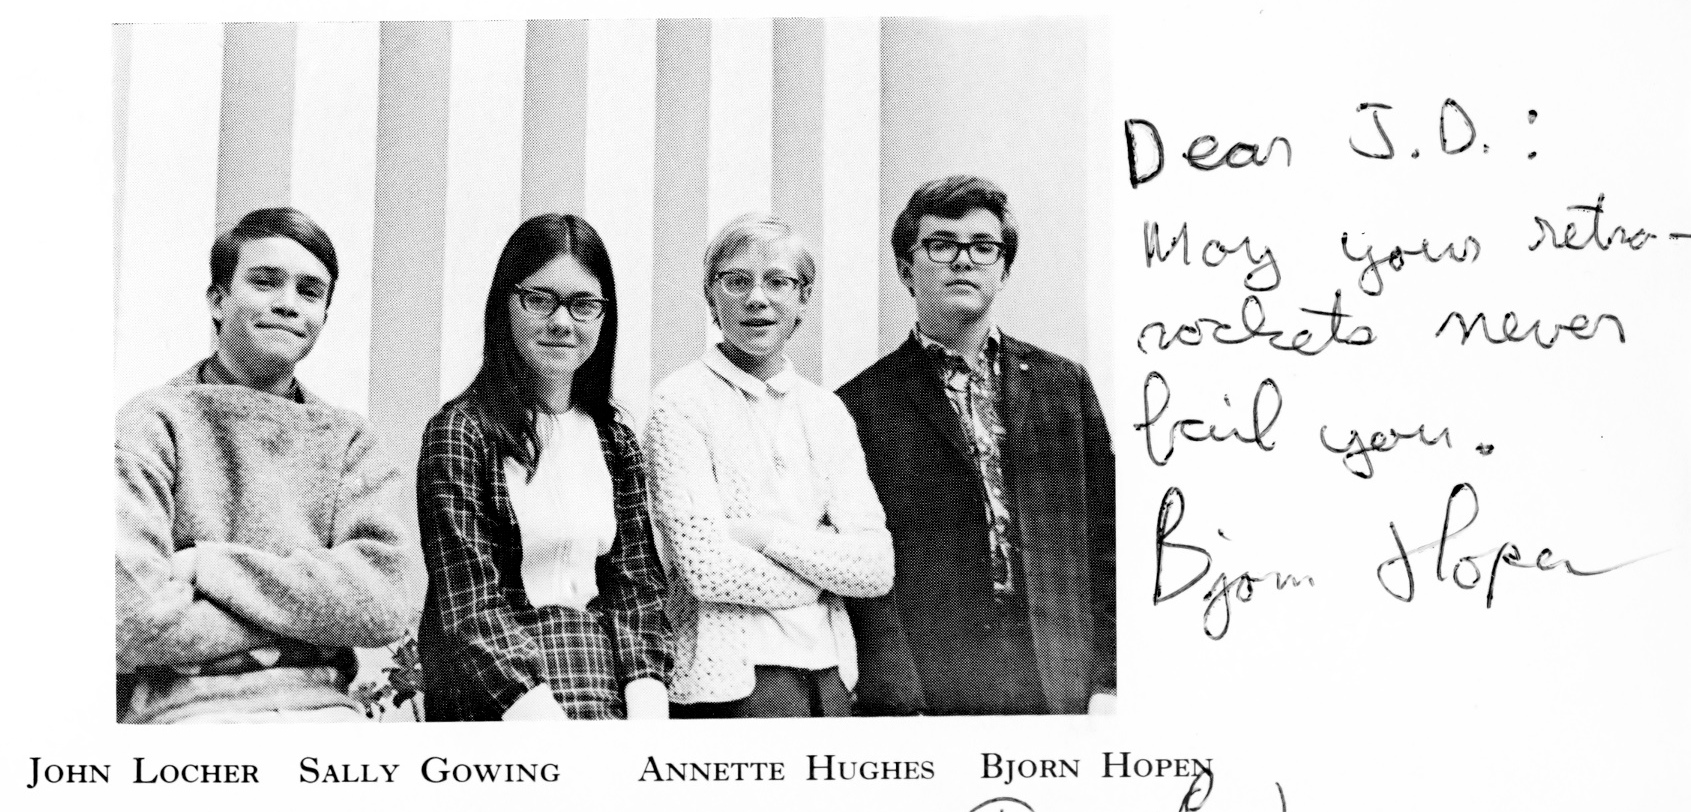
\includegraphics[width=0.50\textwidth]{bjorn_acs_yearbook_1968.jpg}}
\caption[Bjorn Hopen (1954-1970)]{\href{https://www.findagrave.com/memorial/244135118/bjorn_erik-hopen/flower}{Bjorn Hopen (1954-1970)}. Bjorn (the boy on the right with glasses) killed himself the year after I left Beirut.
It was pure adolescent weakness and waste. This is the only image I have
of him. Taken from an old ACS yearbook.}
\label{fig:8196x0}
\end{SCfigure}

Richard was the next to go.

I was much closer to Richard than my other friends. We corresponded for
years after leaving Beirut and traded long-distance phone calls in an
era when long distance wasn't cheap. We both ended up in university. I
went to the University of Alberta, and Richard attended a small college
in Pennsylvania. During our summer break between our third and fourth
years, Richard called me and said he was coming west on a college
geology field trip. Richard once told me that he used to idolize the
American West, at least until he met me! As a Montana boy, I was a bona
fide westerner, but I didn't meet Richard's expectations; it was a
``never meet your heroes'' sort of thing.

We agreed to meet near Mount Rushmore. I had a good summer job working
the oil fields near Slave Lake, Alberta, but it was shiftwork with big
blocks of off time. I took a few days and drove the 1200 miles from
Slave Lake to Rushmore. I did it in one mad butt-numbing all-day and
overnight shot. This was my first trip to Rushmore. In the 1970s,
Rushmore looked like it did in the classic Hitchcock movie \emph{North
by Northwest}. I was impressed. I was even more impressed by the massive
\emph{Crazy Horse Memorial} that is still being carved about twenty
miles from Rushmore.

Richard and I were delighted to see each other. I knew from his letters
and calls that he was struggling. It wasn't his coursework. He was doing
fine in college, better than me, but his social life troubled him. He
was lonely, depressed, and terribly sad that he didn't have a girlfriend
or any close friends. While I sympathized with Richard, his complaints
secretly annoyed me. So life isn't going your way; welcome to the goddamn
club. I didn't voice my annoyance, and Richard was so wrapped up in his
feelings he didn't pick up mine. We stayed up all night talking and
watching the stars from the pitch-black grounds of a small motel near
Rushmore. It was a clear summer night, and the summer triangle stars
were almost lost in the Milky Way's backbone. Early next morning, I left
to drive back to Slave Lake.

I didn't hear from Richard again until he called me in our fourth year a
few weeks before Christmas. He called from a payphone in a US/Canada
border town (I cannot remember which one) and said he was driving to
visit me in Edmonton. It was completely unexpected. He said the Canadian
border officials wouldn't let him in because he carried too much cash. I
told him to try another crossing and lie; it worked. Borders have never
been secure! When he arrived in Edmonton, he had a long story to tell.
In his last year at college, he suffered from severe depression. He was
hospitalized and put on lithium drugs. Depression drugs in the 1970s
sucked. They often did more harm than good, but the treatment seemed to
help him, and in a few weeks, he was discharged. He tried finishing his
degree but couldn't concentrate. Then, suddenly, he decided to see me. I
still don't know why he had to see me. Maybe I made him happy.

His arrival in Edmonton was not convenient. I had no place for him to
stay. I was living in a student cooperative at the time. The cooperative
rented dilapidated houses near the university and stuffed them with poor
students. When Richard showed up, I was the cooperative's treasurer,
meaning I had the delightful chore of collecting rent from all the
little cosplaying student Marxists and Maoists who felt rent should be
free.

``Like, stop suppressing us, man.''

Sadly, for the commies, I was a mean bastard and locked rent delinquents
out of their rooms until they paid up. Until the checks clear, fuck the
revolution! The cooperative was full, so Richard crashed on my room's
floor. He didn't mind, and neither did I. We had a grand time in
Edmonton. He certainly didn't help my grades. I wasted so much time with
Richard that I barely passed my last year. Richard didn't go to school.
He got a job as a night watchman and spent his free time walking around
the city. He was still taking drugs for awful canker sores, and he was
still depressed. It was around this time that Richard fixed his
virginity problem by hanging out in bars and hiring prostitutes. One
weekend he smuggled a whore into the cooperative and did the deed in my
bed. I don't remember how much he paid her, but she did such a good job
he tipped her. Richard was always the gentleman. I was impressed. I
lacked the guts to hire prostitutes; I was always that guy who worried
about venereal diseases. My reticence probably saved my life a few years
later when I had a chance to screw a skinny Ghanaian woman that, when I
think back, probably was suffering from AIDS. After his prostitute
encounter, Richard was tested for VD. He delighted in explaining how the
nurse dipped what sounded like a giant Q-tip in his penis. He didn't
catch anything, which, as it turned out, may not have been a good thing.

One of my best memories of Richard was spending Christmas with him and
my family in Calgary. On my Christmas break, we drove Richard's clunky
old car down to Calgary and stayed with my parents. I remember Richard
was touched by a Christmas gift my mother got him. He almost cried when
she handed him a big, wrapped present. After Christmas, we drove out to
Banff. It was one Canadian place Richard desperately wanted to visit. He
wanted to hike, but it was winter. The snow was deep and magnificent. I
talked him into giving snowshoeing a try. He loved it. Banff was cold,
at least -20C, and the trail we wanted to snowshoe up was
``technically'' closed, but we ignored the trail closure and snowshoed
up Cascade Mountain and slept in -30C weather in a stunning snow-covered
mountain meadow. Snow makes superb cushioning for sleeping bags. I've
never been comfier while camping.

After Christmas, we returned to Edmonton. I resumed my coursework, and a
few weeks into February, Richard decided to return home. I helped him
pack up his car and watched him pull out of the cooperative's driveway.
I was both sad and relieved to see him go. I didn't know it then, but
that would be the last time I'd ever see him.

Without Richard to distract me, I knuckled down just enough to get
through my last term. My grades were mediocre, not good enough to get
into graduate school: once an inferior being always an inferior being. I
didn't know what to do next, but I knew I didn't want to get a serious
job and start adding to the gross domestic product. By sheer luck, I was
recruited by CUSO (basically the Canadian Peace Corps) to teach
mathematics in Ghana. A few months later, I was teaching high school in
Tamale, Ghana. Of all the jobs I've done over a long and embarrassing
career, I liked teaching the best. But sadly, I could make far more
money as a programmer than I ever could as a teacher. So instead of
putting up with undermotivated horny teenagers, I put up with corporate
fools and tools instead. ``Work,'' for me, remains a four-letter word.

Near the end of my second term in Tamale, I got a letter from Richard's
mother. I once met Richard's mom in Beirut. She was a bit older than my
mother and a lovely woman. She took Richard and me to a nice Beirut
restaurant, a nice break from our grim dormitory gruel. I could tell
from her handwriting on the envelope that it was bad news. I opened her
letter and read that Richard had killed himself by firing a shotgun into
his head! Like Bjorn, he had rented a room, checked in, and then checked
\emph{way} out. But, unlike Bjorn, Richard didn't opt for pussy boy
sleeping pills; he made sure he wouldn't survive by using a shotgun. As
I read Mrs. Moore's letter, I started shaking. I was surprised by my
body's reaction to Richard's death. Why am I feeling like this?

I took a day off teaching and tried to answer Mrs. Moore's letter. She
was begging me for details about our time together in Edmonton. She was
grasping for anything that might help her understand her son's death.
She was also very worried about her husband. Richard and his dad were
very close. Whenever Richard spoke about his dad, it was with unusual
affection. I respected and admired my dad, but I didn't have the same
connection with him that Richard had with his father. Richard's suicide
had deeply, deeply hurt Mr. Moore. Mrs. Moore was probably thinking she
might have to deal with a double suicide. I sat on Mrs. Moore's letter
for a few days but never replied. The days turned into weeks, and I
still didn't reply. She even sent me a follow-up letter, to which I also
never replied. It's still one of the least considerate and cruel things
I have ever done, and trust me, I am a vicious lifelong asshole.
\href{https://www.findagrave.com/memorial/162651768/richard_william-moore}{Richard
was twenty-two} when he killed himself.

% captions beside figure
\captionsetup[figure]{labelformat=empty}
\begin{SCfigure}
\centering
\href{https://conceptcontrol.smugmug.com/People/Inlaws-Outlaws-and-Friends/i-dNPP9pn/A}{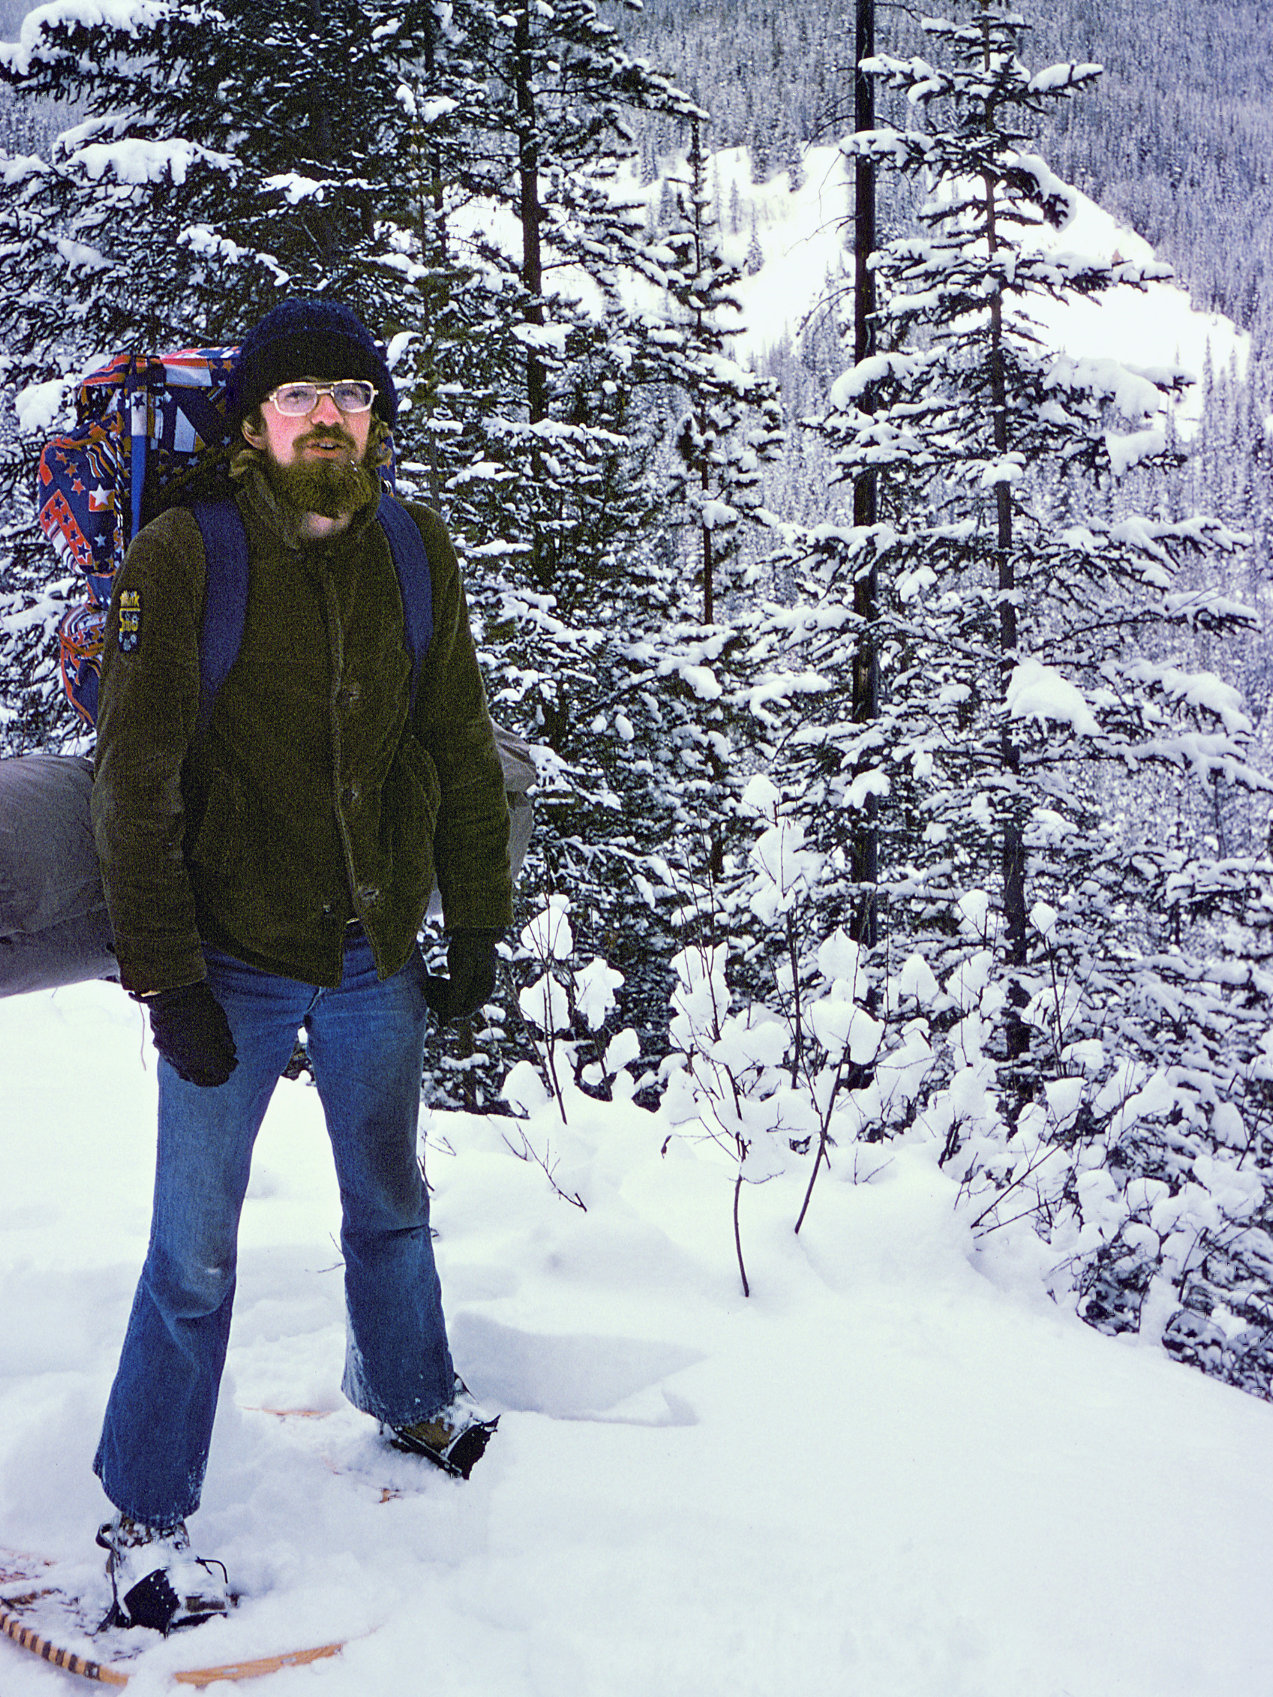
\includegraphics[width=0.40\textwidth]{richard_moore_banff_1974.jpg}}
\caption[Richard Moore (1953-1976)]{\href{https://www.findagrave.com/memorial/162651768/richard_william-moore}{Richard
Moore (1953-1976)} in the mountains above Banff in western Canada. This
was our last trip together. We forced our way up the Cascade trail on
snowshoes and camped in -30C weather. Within a few months, I was
teaching mathematics in Ghana, and Richard was being treated for
depression for the second time.}
\label{fig:8196x1}
\end{SCfigure}

Ned was the next to go.

Ned was the most curious and mathematically gifted of us. Even at ACS,
he was years ahead of everyone in math, but despite his brilliance, Ned
was a troubled child. When I met Ned, he lived with his bitterly
divorced father in Beirut. Ned's dad had some affiliation with the
American University of Beirut (AUB). When his marriage collapsed, he got
Ned. I always wondered if Ned's mother didn't want him because his
father didn't behave like a man who had fought for custody. Ned's dad
neglected him. You could tell by Ned's body odor. Ned was often dirty;
you could smell him coming. He also had appalling dental hygiene and
wore ratty clothes that were two or more sizes too small. Once, when we
were sneaking down to the cornice (the Mediterranean Sea was just down
the street) to dip our toes in the surf, I noticed that Ned's shoes had
holes in both soles.

Being neglected wasn't all bad. Ned roamed all over Beirut, and I often
accompanied him. Ned was a day student; he lived in Beirut and could go
anywhere. Bordering students like me were supposed to stay \emph{in
bounds}. School bounds delimited a small section of supposedly safe
streets within easy walking distance of the school. I ignored bounds
along with many other rules. Rules are for the weak, fat, and stupid;
they still are. On one of our \emph{out-of-bounds} outings, Ned and I
were caught shoplifting books. Hey, a boy must read. I was punished by
being put on \emph{D-Pro}.~ ACS had a graded disciplinary system that
mirrored its academic groups. If you were a super good little boy, for
six interminably long weeks, i.e., no demerits, no sneaking around after
lights out, no getting caught off bounds, and so on, you got promoted to
\emph{A}-class. \emph{A}-class kids enjoyed a few privileges like
staying up a little later or studying in their rooms instead of in study
hall. If you broke the odd rule, and who hasn't, you stayed in the
default \emph{B}-class. If you were a little bad, you would be slotted
into \emph{C}-class. If you broke many rules, you were punished in
\emph{D}-class, and if you were a beyond-the-pale juvenile delinquent,
you were put on \emph{D-Pro}. While on \emph{D-Pro,} you were confined
to your room except for classes and meals. I spent months on
\emph{D-Pro} during my Beirut years. Why be a good little boy for months
to earn meager privileges when you can just break the rules and do
whatever the hell you want? I believe I set a record for the longest
time anyone was on \emph{D-Pro} without being expelled. I was a cunning
delinquent. The school had strict rules about drinking and drugs.
Students were immediately expelled if they were caught with either, but
there were no rules about blowing holes in walls with homemade bombs --
more about the bombs later. I forced ACS to expand its rule book. It was
my greatest achievement. Ned was often in on my shenanigans, and our
misadventures had a definite \emph{Huckleberry Finn} vibe.

We used to climb into the attics of AUB buildings and time the fall of
stones to the courtyards below. Ned was checking Newton's \(16t^{2}\)
acceleration due to gravity equation. The math checked out. On another
occasion, we got ahold of old mechanical calculators. Ned found a shop,
off bounds, of course, that sold office calculators. In 1968, office
calculators were gigantic gear-laden metal dragons. They looked like
typewriters on steroids. The shop owner didn't mind weird little
American kids computing cube roots on the clanky old machines. Ned posed
problems that sent the beasts into infinite gear-grinding loops. Loops
were a lot more fun in the days of motors and gears.

What I most admired about Ned was that he honestly did not give a
ding-dong damn about what others thought about him. I'm sure the girls
in our classes noticed his body odor, old clothes, and unkempt hair and
said the usual mean teenage girl shit behind his back and maybe even to
his face. He didn't care. Ned even blew off our gym instructors, who
took unseemly homoerotic pleasure in forcing us into the showers. Ned
wouldn't have it. He went to class all sweaty and smelly. Oh, he'd get
punished, but that didn't faze him. He also didn't give a shit about his
dad's edicts. He ignored his dad like I ignored bounds. Ned was a
20th-century \emph{Huckleberry}.

I've already noted that Ned's letters were the best. They were little
masterpieces. No topic was taboo. One of his missives outlined his
masturbation experiments. He was on a perfect orgasm quest. Another
tediously exhibited a long PL1 program -- his favorite programming
language -- that efficiently implemented the \emph{Newton-Raphson}
method. Other letters included cartoon clippings and photographs. Ned
started developing 35mm black and white negatives after I left Beirut.
In a bit of synchronicity, I also got into developing 35mm black and
white negatives in Edmonton. We compared techniques, and for the first
time, I found something I was better at than Ned. Ned's letters were
better than social media and it pains me that I didn't keep them. We
corresponded a few years after I left Beirut, but then Ned dropped off.
We stopped trading letters. Maybe it was my fault. Maybe it was his. We
were both moving on. Ned, as I mentioned earlier, went to MIT with
David.

I didn't hear about Ned again until David called after the 9/11 attacks
in New York. David and I had reestablished contact via email after
decades. We had a good long chat about 9/11 and -- oddly -- Ned. David
didn't buy the official 9/11 story. He couldn't believe a small group
could pull off such a stunt. He didn't go down the fire \emph{doesn't
weaken steel beams} (it does) rabbit hole or buy the \emph{controlled
demolition} (it wasn't) nonsense, but he couldn't accept that the
government could be so inept. In 2001, I was a jaded cynic. I was
confident that the US government couldn't find its butthole with two
hands and a flashlight. My stance has only hardened. Now I doubt they
could manage it with a search party and butthole sniffing dogs. The US
government has repeatedly demonstrated that it is capable of
awe-inspiring stupidity. 9/11 magnitude fuckups are what I expect from
these clowns. Just ask the guys who fell off that plane bugging out of
Kabul.

David filled me in on what he knew about Ned. Ned started at MIT the
same year as David but didn't adapt well. He dropped out in his second
year and disappeared. David lost track of him and learned years later
that he had ended up in Stillwater, Oklahoma, living with his sister.
Ned had some role at the University of Oklahoma, either as a tutor or a
nonacademic staff member, and was still futzing around with prime
numbers. He never married, had no close friends, and lived like a
homeless person \emph{in a house}. Ned's sister contacted David when Ned
suddenly died of a heart attack.
\href{https://www.findagrave.com/memorial/11932084/edwin_terry-prothro}{Ned
was fifty-one} when he died. Ned should have done better in life. He had
gifts. He wasn't depression-prone like Richard, and he had chances; he
just didn't seize them. I was surprised and saddened to learn of Ned's
death. His life ended just as mine was kicking into a better and happier
phase.

% captions beside figure
\captionsetup[figure]{labelformat=empty}
\begin{SCfigure}
\centering
\href{https://conceptcontrol.smugmug.com/Places/Overseas/Beirut-Lebanon-1960s-1/i-sG6bVnH/A}{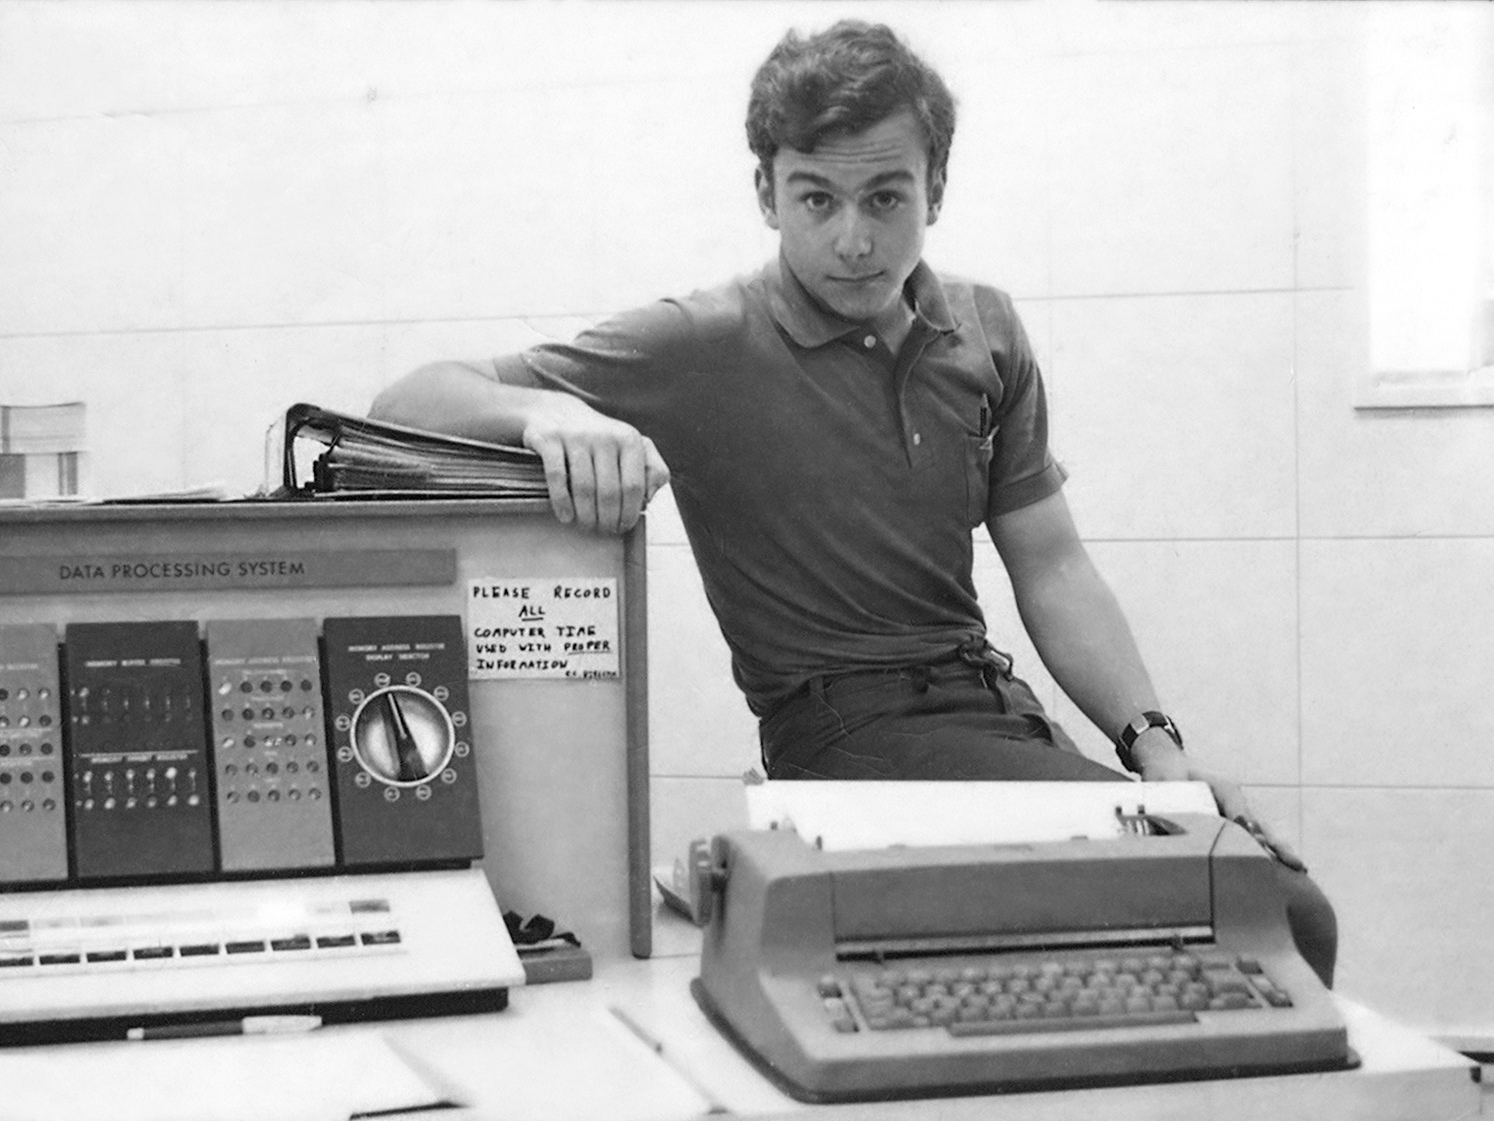
\includegraphics[width=0.50\textwidth]{ned_prothro_by_computer_1970.jpg}}
\caption[Ned Prothro (1953-2004)]{\href{https://www.findagrave.com/memorial/11932084/edwin_terry-prothro}{Ned
Prothro (1953-2004)} was one of my best friends at ACS in Beirut. He
went to MIT, dropped out, and ended up in Stillwater, Oklahoma, where he
lived until his untimely death of a heart attack at the age of 51.}
\label{fig:8196x2}
\end{SCfigure}
 

This finally brings us to David. As I said, David died in February of
2024 at seventy. For the last few years, David's health has been awful.
I only learned of his problems because I was in the habit of sending
David yearly emails asking if he was still alive. Two years ago, there
was no response to my email, but a few months after sending it, David
and his wife, Caryn, called. They told me about his health problems. He
had been bedridden for weeks and could barely move his arms. He couldn't
work his computer and thus could not respond to emails. I don't know
what he suffered from. I'm not sure if even David knew. After hearing
this news, I decided to ping him every six months to see how he was
doing.

David was by far the most successful of our little clique. Unlike Ned,
he navigated the rigors of MIT and graduated with an Electrical
Engineering degree. After graduating, he married Caryn. Caryn is blind.
Her blindness did not prevent them from having kids and enjoying family
life. Caryn's blindness also positively impacted David's career.
Together, they founded a software company that specialized in Braille
printing. With David's specialized software, blind people can print and
read computer text. His software is still used worldwide, and I have no
doubt it has helped many people. Good for you, David! David's
achievements were noteworthy enough to
\href{https://en.wikipedia.org/wiki/David_Holladay}{merit a Wikipedia
Page}. Take a look; he was a genuine \emph{mensch}.

Now for that trauma that David and I shared.

In 1968, the last half of my second Beirut year, David, a day student
like Ned, came to school with a small bomb he had made by slicing open
firecrackers with razor blades and pouring the gun powder into a small
chemistry set glass bottle. David was proud of his bomb. He had even
printed a label ``Bomb Zero'' (David was into zero-origin indexing) that
he had glued to the glass bottle. We all admired his work and
immediately started looking for something to blow up.

We found a crack in a concrete wall surrounding one of the school's
playgrounds. The bomb fit snugly in the crack. We waited until the coast
was clear, then Ned, Richard, David, and I took the bomb outside, placed
it in the crack, and lit its long gangly fuse. With the fuse lit, we all
ran. I ran parallel to the wall while the others ran perpendicularly;
they were putting themselves in greater danger. I remember thinking,
``What the fuck, guys,'' as I fled. The bomb detonated with a huge bang
that echoed off the buildings around the playground. Everyone was far
enough away to avoid injury. We returned to the blast site and inspected
the damage. David's bomb had blown a two-foot hole right through the
concrete wall. We took turns poking our heads through the hole and
enjoying the view of the other side.

The bomb was, forgive me, a blast. And, just to be clear, our gang was
setting off bombs in Beirut long before Hezbollah and the Israelis.

When teenage boys do something spectacularly stupid, and it works out,
do they conclude, ``Well, that was idiotic -- never again?'' No, teenage
boys resolve to do something even stupider. After ``Bomb Zero's'' big
blast, we decided an encore was mandatory, so we spent the next week
walking around Beirut scouring shops for firecrackers. Then Ned,
Richard, David, and I went to David's parents' apartment and started
slicing open dozens of firecrackers with razor blades and pouring the
fine black powder into ``Bomb One's'' glass bottle.

While we were pouring powder, Ned had the insane idea of putting a coin
in the bottle. He wanted to see what the blast would do to it. So, in
went the coin, which David, the master bombmaker, tamped down with a
small metal rod. As David handled the bomb, I remember leaning down to
get a better look. In the last second, David raised his left arm,
blocking my view, as ``Bomb One'' loudly detonated in his bedroom. The
next instant, I was on my knees facing the other way. My eyes were
tightly shut, and I remember calmly thinking, ``Well, I'm going to open
my eyes and see if I can see.'' I opened my eyes; they still worked.
Good. I looked up at Richard. His thick glasses were frosted with glass
pellets, and his forehead was bleeding. Ned, who had been the furthest
away, looked like a ghost. His face was blanched white, and his big dark
eyes were wide and shocked. My ears were ringing, and the smell of burnt
powder was everywhere. I got to my feet and headed out the bedroom door.

In the hallway, I saw David rush by holding a mangled, bleeding hand. I
didn't know how badly he was hurt, but he was spraying blood all over
the hall. Lucky for us, an older girl, I forgot who was present. She
came running when she heard the blast and had the presence of mind to
wrap David's hand in a towel and rush him to the hospital.

Ned, Richard, and I left the apartment, not knowing what to do, but we
all knew we were in super deep shit. I can remember aimlessly wandering
around Beirut streets until our ears stopped ringing. We were relieved
we could hear again. Then, I noticed something was wrong with one of my
eyes. We found a restroom with a mirror, where I found a small glass
fragment in my right eye. I knew then that David's last-second arm
movement had saved my eyesight. The shower of glass particles that
Richard's thick glasses had stopped would have gone right into my face
if David's arm had not occulted the blast. For months afterward, David
pulled tiny shards of glass out of his left arm.

I was taken to an eye specialist after discovering the glass fragment in
my eye. I had eye surgery in the AUB hospital that left a small
vision-obscuring scar on my right cornea. Even now, fifty-six years
after the blast, the scar still slightly blurs my right eye. It's been a
lifelong reminder of my paramount \emph{dumbfuckery}. As for David, the
blast tore off the tips of his right hand's thumb and two fingers. I'm
sure David thought of the bomb every time he did anything that required
two thumbs. His mangled hand was David's lifelong reminder of \emph{his}
paramount \emph{dumbfuckery}.

After our respective surgeries, David and I spent a few days in the same
Beirut hospital room. Then, it was back to school, where I joined
Richard on \emph{D-Pro}. We were all punished. Richard and I were
incarcerated for the rest of the term on \emph{D-Pro,} while Ned and
David, both day students, were banned from campus except for class
hours. The bomb did not end our friendships; it strengthened them.
During our \emph{D-Pro} incarceration, Richard and I chiseled a small
hole in the wall that separated our rooms so we could talk to each
other. In our second year, the school separated us; we were too
much trouble together. They put us back together in our third year,
probably because they didn't want to repair any more wall holes. Ned
used his campus banishment to wander further afield in Beirut, and David
enjoyed an unexpected notoriety showing off his skin-grafted fingers.
Before the bomb blew off David's fingers, girls ignored him. Afterwards,
he was a chick magnet. I was jealous.

\captionsetup[figure]{labelformat=empty}
\begin{SCfigure}
\centering
\href{https://conceptcontrol.smugmug.com/Places/Overseas/Beirut-Lebanon-1960s-1/i-4v89f4D/A}{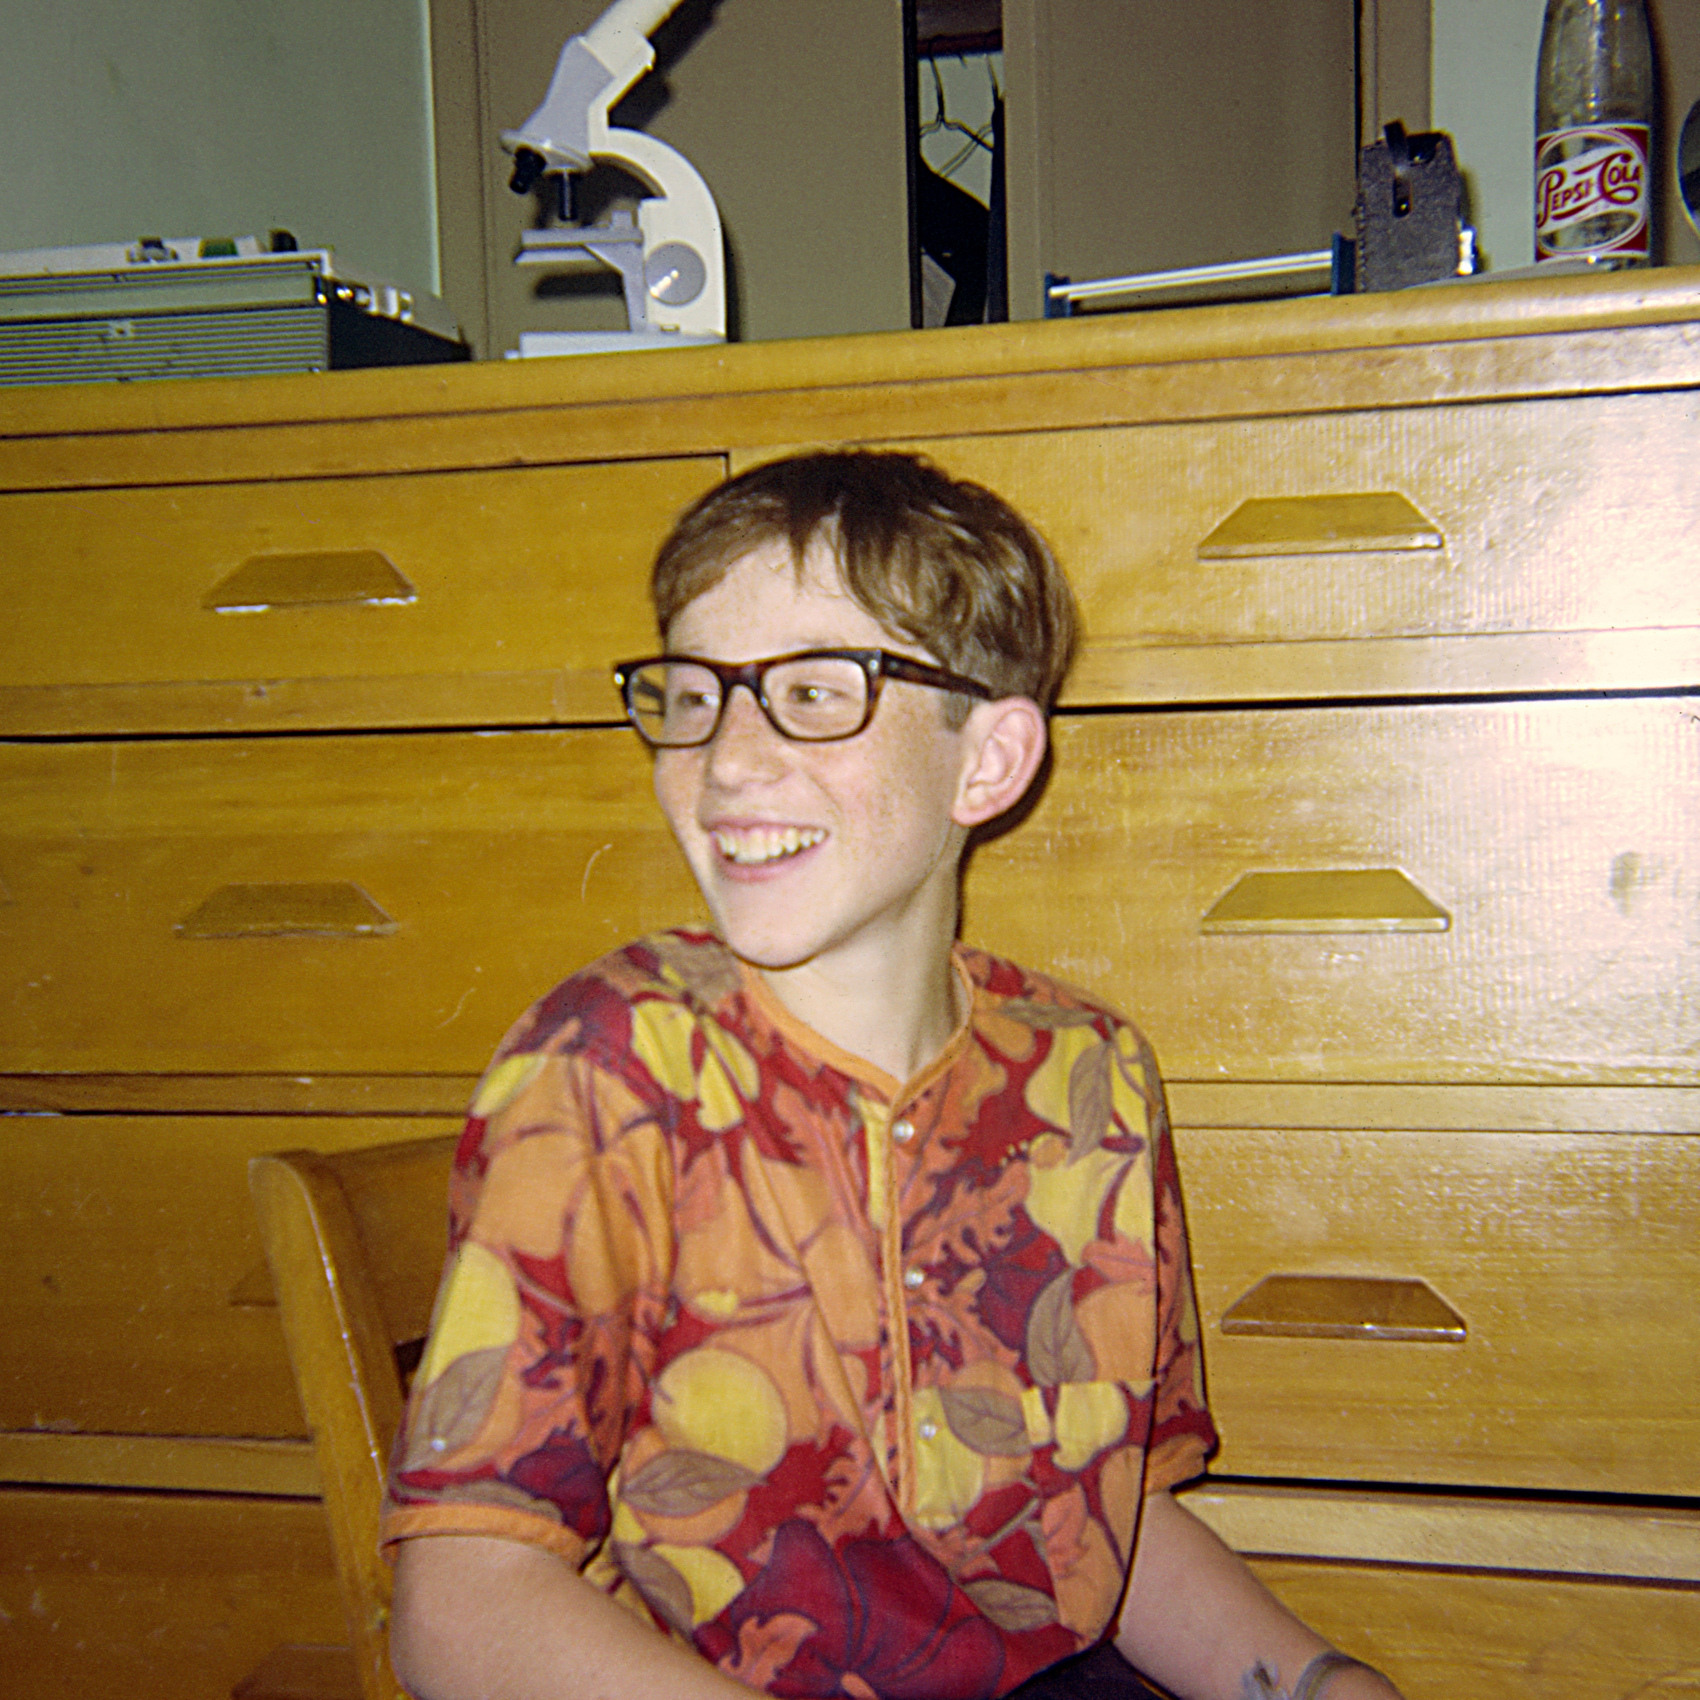
\includegraphics[width=0.40\textwidth]{david_holladay_acs_dorm.jpg}}
\caption[David Holladay (1953-2024)]{\href{https://en.wikipedia.org/wiki/David_Holladay}{David Holladay (1953-2024)} in my dorm room at the ACS American Community
School in Beirut, Lebanon.}
\label{fig:8196x3}
\end{SCfigure}

Honestly, I was jealous of all my ACS friends. I felt they were all
smarter and destined for great things, but life didn't go as expected,
especially for me, the last schoolboy standing.

%\end{document}

